\UseRawInputEncoding
\documentclass[conference]{IEEEtran}
\IEEEoverridecommandlockouts
% The preceding line is only needed to identify funding in the first footnote. If that is unneeded, please comment it out.
\usepackage{cite}
\usepackage{float}
\usepackage{amsmath,amssymb,amsfonts}
\usepackage{algorithmic}
\usepackage{graphicx}
\usepackage{textcomp}
\usepackage{xcolor}
\usepackage{booktabs}
\usepackage{siunitx}
\usepackage{listings}
\usepackage{xcolor}
\usepackage{subfigure}
\usepackage{url}
\usepackage{xurl}% Required for \url command
\def\BibTeX{{\rm B\kern-.05em{\sc i\kern-.025em b}\kern-.08em
    T\kern-.1667em\lower.7ex\hbox{E}\kern-.125emX}}

% ---------- Arduino language definition ----------
\lstdefinelanguage{Arduino}{
  language=C++,                       % inherits C++ rules
  morekeywords={digitalWrite, digitalRead,
                pinMode, analogRead, analogWrite,
                INPUT, OUTPUT, HIGH, LOW, delay},
  morecomment=[l]{//},                % line comments
  morecomment=[s]{/*}{*/},            % block comments
  morestring=[b]"                     % strings
}

% ---------- Global listing style ----------
\lstset{
  language=Arduino,
  basicstyle=\ttfamily\scriptsize,    % use script‑size to fit two‑column
  numbers=left,
  numberstyle=\tiny,
  stepnumber=1,
  frame=single,
  breaklines=true,
  columns=fullflexible,
  keywordstyle=\color{blue!70!black},
  commentstyle=\color{gray!60},
  stringstyle=\color{orange!80!black},
  captionpos=b                        % caption under listing
}





\begin{document}

\title{A Sweat-Based Wearable Sensor for Real-Time Lactate and Glucose Monitoring in Endurance Athletes}

\medskip

\author{\IEEEauthorblockN{Elliot Metcalf}
\IEEEauthorblockA{\textit{Department of Electrical and Computer Engineering} \\
\textit{Rice University}\\
Houston, USA \\
etm2@rice.edu}
\and
\IEEEauthorblockN{Priyanka Amalkar}
\IEEEauthorblockA{\textit{Department of Electrical and Computer Engineering} \\
\textit{Rice University}\\
Houston, USA \\
pa52@rice.edu}
\and
\IEEEauthorblockN{Zhenya Liu}
\IEEEauthorblockA{\textit{Department of Electrical and Computer Engineering} \\
\textit{Rice University}\\
Houston, USA \\
zl181@rice.edu}
}

\maketitle

\begin{abstract}
This project explores a sweat-based wearable sensor for real-time monitoring of lactate and glucose in endurance athletes during training. Monitoring these analytes enable athletes  to optimize workout intensity levels and recovery, leading to enhanced overall performance. Current commercial tracking solutions are invasive (blood-based), expensive, and unsuitable for continuous monitoring, leading to undesired disruption during activity. To address these limitations, the design team conducted extensive research on existing sweat-based sensing devices and developed an outline of a wearable system that integrates a custom sensor, a flexible circuit board, and microfluidic channels. The system can interact with a smart watch or smartphone via Bluetooth, providing athletes with near-real-time biochemical feedback.

\end{abstract}

\smallskip

\section{Introduction}
During endurance and sports training, it is important to track different analytes to determine physiological changes [1]. Knowing the impact of these fluctuating biomarkers, such as glucose and lactate, can reveal ways to enhance athlete performance. Lactate levels are key for athletes to track since increasing levels are indicative of anaerobic metabolism, which causes muscle fatigue and cramping. Determining their lactate threshold allows the athlete to understand their optimum training and monitor fatigue to improve performance [2]. Glucose is another important analyte to track since decreasing glucose levels directly correspond to decreasing energy levels. Alerting the athlete when their blood sugar decreases will allow them to time their food intake to maintain stable energy levels throughout the training session [3]. 
Although sweat sensors to measure glucose and lactate have been in the works, our proposed system is unique in that our target users are athletes. Because sweat compositionally varies when induced in different circumstances (exercise, thermal, emotional induction) our team decided to focus on exercise-induced sweat, which mostly originates from the eccrine glands.  The differences are mostly due to local blood flow, metabolic activity, and sympathetic stimulation of the glands. Lactate levels are higher exercise-induced sweat, while glucose levels are lower, which would require our sensor to be optimized for those particular concentration ranges of the analytes [4]. 

\bigskip

\section{Method}

\subsection{Device}
The methodology for developing our wearable biosensor device involved a multidisciplinary, iterative design process including sensor fabrication and the integration of a flexible PCB with a microfluidic patch for real-time analyte monitoring. The system supports three-electrode electrochemical measurements, sweeping the potential in both anodic and cathodic directions at defined rates (mVs$^{-1}$) to probe oxidation and reduction reaction characteristics. The proposed device integrates an Arduino Uno R3 microcontroller for both parameter control and data acquisition and a potentiostat circuit. It runs a sketch (Appendix.\ref{prototype}), enabling us to conduct a cyclic voltammetry test by specifying the initial potential, vertex potential and scan rate. A potentiostat is able to maintain a set potential difference between a working and a reference electrode with operational amplifiers while the electrodes are submerged in solution. Constructing a basic potentiostat requires several standard components: resistors, capacitors and operational amplifiers. Fig.\ref{fig1} shows the circuit diagram of our potentiostat circuit. It could be divided into excitation chain and acquisition chain for voltage control and current sensing. Input to excitation chain (Fig.\ref{fig16}) simulated with a pulse width modulation (PWM) signal due to the fact that Arduino Uno R3 lacks a true DAC. It is routed through a second order RC filter with it's noise ripples being filtered out. The filtered output follows with a quasilinear ramp from 0 to 5V and is designed to drive the three-lead electrochemical cell after being scaled and centered to \textpm1V. The smallest step is approximately 7.8mV (256 levels across \textpm1V) on the electrodes. The PWM frequency was modified to approximately 31.4 kHz in Appendix.\ref{prototype} by changing the divider factor to 1 in Equation (1), where the clock frequency for Arduino R3 UNO board is 16 MHz. 

\begin{equation} f_{PWM} = \frac{f_{clk}}{N_{div}2^n}, \; f_{clk} = 16MHz, \, n = 8,\, N_{div} = 1,\end{equation}

\begin{table}[ht]
  \centering
  \begin{tabular}{|l|c|r|}
    \hline
    \textbf{Input PWM level} &  \textbf{Input voltage(V)} &\textbf{$v_{\mathrm{out}}$ (V)} \\ 
    \hline
    0   & 0&  1  \\
    127 & 2.5&  0  \\
    255 & 5& –1  \\ 
    \hline
  \end{tabular}
  \caption{Truth table for the excitation chain}
  \label{tab1}
\end{table}

The acquisition chain (Fig.\ref{fig17}) containing a transimpedance amplifier converts the current flow on the counter electrode to voltage. As Tab.\ref{tab2} suggests, the output was centered on mid-supply, allowing the 10-bit ADC on the Arduino Uno R3 to quantify the entire \textpm 200$\mu\text A$ range dynamically. The current is limited by the resistor $R_{5}$ connected to the transimpedance amplifier feed back loop. And according to the property of operational amplifiers and Ohm's law, the current limit is given by: 

\begin{equation} V_{in} = i_{CE}\;\times \;R_{5}\end{equation}
Where $V_{in}$ is the converted voltage output. The potentiostat was optimized to span the Arduino Uno's full 0-5V ADC range due to it can not measure negative voltages. By dividing the voltage measured at teh series port by $R_{5}$ and plotting the resulting current versus the applied potential sweep, the cyclic voltammetry response can be directly obtained. Bench test was conducted in a 0.1M Phosphate-Buffered Saline (PBS) solution spiked with 30\% hydrogen peroxide ($H_2O_2$) using Metrohm 110 three-lead electrochemical sensor. 

\begin{table}[ht]
  \centering
  \begin{tabular}{|l|c|r|}
    \hline
    \textbf{$i_{\mathrm{CE}}$ (uA)} &  \textbf{Output $v_{\mathrm{in}}$} &\textbf{ADC level} \\ 
    \hline
    -200   & 0&  0  \\
    0 & 2.5&  511  \\
    200 & 5& 1023  \\ 
    \hline
  \end{tabular}
  \caption{Truth table for the acquisition chain}
  \label{tab2}
\end{table}



\subsection{Sensor}
The sensor consists of a reference electrode, two working electrodes (for lactate and glucose detection), and a counter electrode. The reference electrode provides a stable potential, the working electrode detects changes in current caused by the redox reactions, and the counter electrode completes the circuit by undergoing the opposite reaction [5].
Manual screen printing was chosen to prototype the sensor because it enables quick iteration and reprinting if design changes are made. Silver ink is used for the traces and the reference electrode due to high conductivity and low resistance [6]. Carbon ink is used for the working electrodes because the rough surface promotes better enzyme immobilization and does not oxidize easily [7]. 
The electrochemical biosensor operates by detecting changes in current caused by redox reactions that have been catalyzed by the respective enzymes specific to the two target analytes. For glucose detection, the enzyme glucose oxidase was chosen, and for lactate detection, lactate oxidase was chosen. Both reactions reduce oxygen to yield hydrogen peroxide (H2O2). Prussian blue is another component to the sensor that is deposited onto the working electrodes and is a transducer of H2O2, allowing its selective reduction [8]. The current from this reduction reaction is directly proportional to the concentration of analyte in the sweat. A potentiostat is used to maintain a set voltage between the counter and working electrode, relative to the reference electrode, by adjusting current levels at the counter.
The printed sensor design shares a single counter and reference electrode between the two working electrodes. To ensure uniform current distribution, the working electrodes are equidistant from the counter electrode. The counter electrode and internal reservoir area were constrained to 11mm by 5mm to minimize reservoir volume and time to collect sweat. The final working electrode diameters will be optimized based on calibration testing.
The manual screen-printing process involves layering Kapton adhesive onto a clear PET (acetate) base. A Cricut machine etches the design onto the substrate, exposing the silver areas. The silver ink is applied and cured at 120 Celsius for 15-20 minutes. Next, the carbon printing areas are exposed, and a layer of carbon ink is applied with a slight overlap onto the silver traces to ensure connectivity. The sensor is then cured again at the same temperature and time period.
To verify electrical connectivity of the sensor, resistance testing was conducted across the silver and carbon ends of the working and counter electrode. A reading of 1 kOhm or lower should be achieved because the small concentrations to be measured from the sweat require higher sensitivity, therefore low resistance in the electrodes. Failures of this test may be attributed to gaps or lifting in ink during fabrication. About half the sensors passed this test in each batch.
To protect the electrodes and prevent unwanted reactions during CV with distorted results, an isolation solution was prepared from the thermoplastic elastomer Styrene Ethylene Butylene Styrene (SEBS) dissolved in tetrahydrofuran (THF). Resistance was retested and three-quarters of the remaining sensors passed the test. 
Cyclic voltammetry was conducted using phosphate buffered saline (PBS) due to its similarity of salt and pH to biofluid composition. A successful CV test displays the characteristic prussian blue redox peaks, negative peak during reduction and positive peak for oxidation, confirming the sensor’s functionality. Distorted CV test results display multiple peaks, likely due to side reactions from unintended electrode exposure.
After prototyping, the inkjet FujiFilm Dimatix printer was used to print the sensors with slightly modified carbon and silver inks to printer specifications. The modified carbon ink did not contain prussian blue, so it needed to be electrochemically deposited onto the working electrode using cyclic voltammetry. The deposition amount is confirmed by observing the redox behavior of the iron ions. Similarly, nickel is also deposited using CV as a protective layer on the PB. 
Next steps for the sensor include enzyme immobilization onto the surface of the working electrodes so a calibration curve can be generated using chronoamperometry. Concentrations of analyte will be incrementally increased to measure current change while maintaining constant potential. This data can be used to characterize sensor performance metrics such as sensitivity and detection limit, as well as how other factors, like differences between people in sweat composition, humidity, and cross-contamination, play a role in the signals generated. Because lactate levels in sweat are high, between 26-136mM lactate in exercise sweat [9], the lactate sensor must avoid signal saturation and handle higher current outputs. In contrast, glucose concentrations in sweat are much lower, between 0.06-0.11mM [4], so the sensor must be highly sensitive and have lower detection limits. Separate calibration curve ranges must be generated for each analyte.


\subsection{Microfluidics}
A microfluidic system was designed to transport sweat from the user's skin to the glucose and lactate sensor for measurement. The initial microfluidic layout was created using AutoCad and the layout was based on our research of microfluidic systems in similar devices [10], [11]. To assess whether the layout was suitable for our project, SimScale was used for computational fluid dynamics (CFD) simulations using the parameters listed in Appendix D. These simulations modeled expected sweat flow behavior through the channels and the reservoir and highlighted areas where adjustments were needed.
Following sensor modifications, in which the electrodes were reconfigured into a smaller elliptical shape, the microfluidic patch layout was refined to improve the rate of fluid delivery and accommodate sensor integration. After each design modification, further simulations were conducted to validate the changes and ensure consistent flow across the sensing reservoir.
Three different designs were chosen for testing, including a single-inlet, dual-inlet, and four-inlet architecture. The molds of these layouts were fabricated using a resin-based 3D printer, and are shown in Fig.\ref{fig13}. Polydimethylsiloxane (PDMS) was then prepared by mixing the polymer base and a curing agent in a 20: 1 ratio, then poured over the 3D printed mold and cured at 70 ° C for three hours to form the microfluidic chip. Two approaches were used to obtain the PDMS chips from the molds, as we anticipated difficulties working with an extremely thin layer of PDMS. The first mold was made with an excess height, and the amount of PDMS required to fill it to a height of 300 microns was calculated and poured in. The second mold had no excess height. PDMS was applied over the mold and a scraper was used to evenly distribute it over the entire surface. An alternative approach, simply printing the microfluidic patch using the 3D printer, was also used. The single and dual inlet designs were successfully fabricated using this approach and then tested using a syringe pump. The syringe pump, depicted in Fig.\ref{fig14}, was set to a flow rate of 0.25 microliters per hour to replicate the sweat rate during intense exercise. Dyed water was used in the testing phase as an analogue of sweat. The lengths of time taken for the water to fill the inlets, reach the reservoir, fill the reservoir, and exit the patch, were measured and compared with target metrics.

\begin{figure}[H]
    \centering
    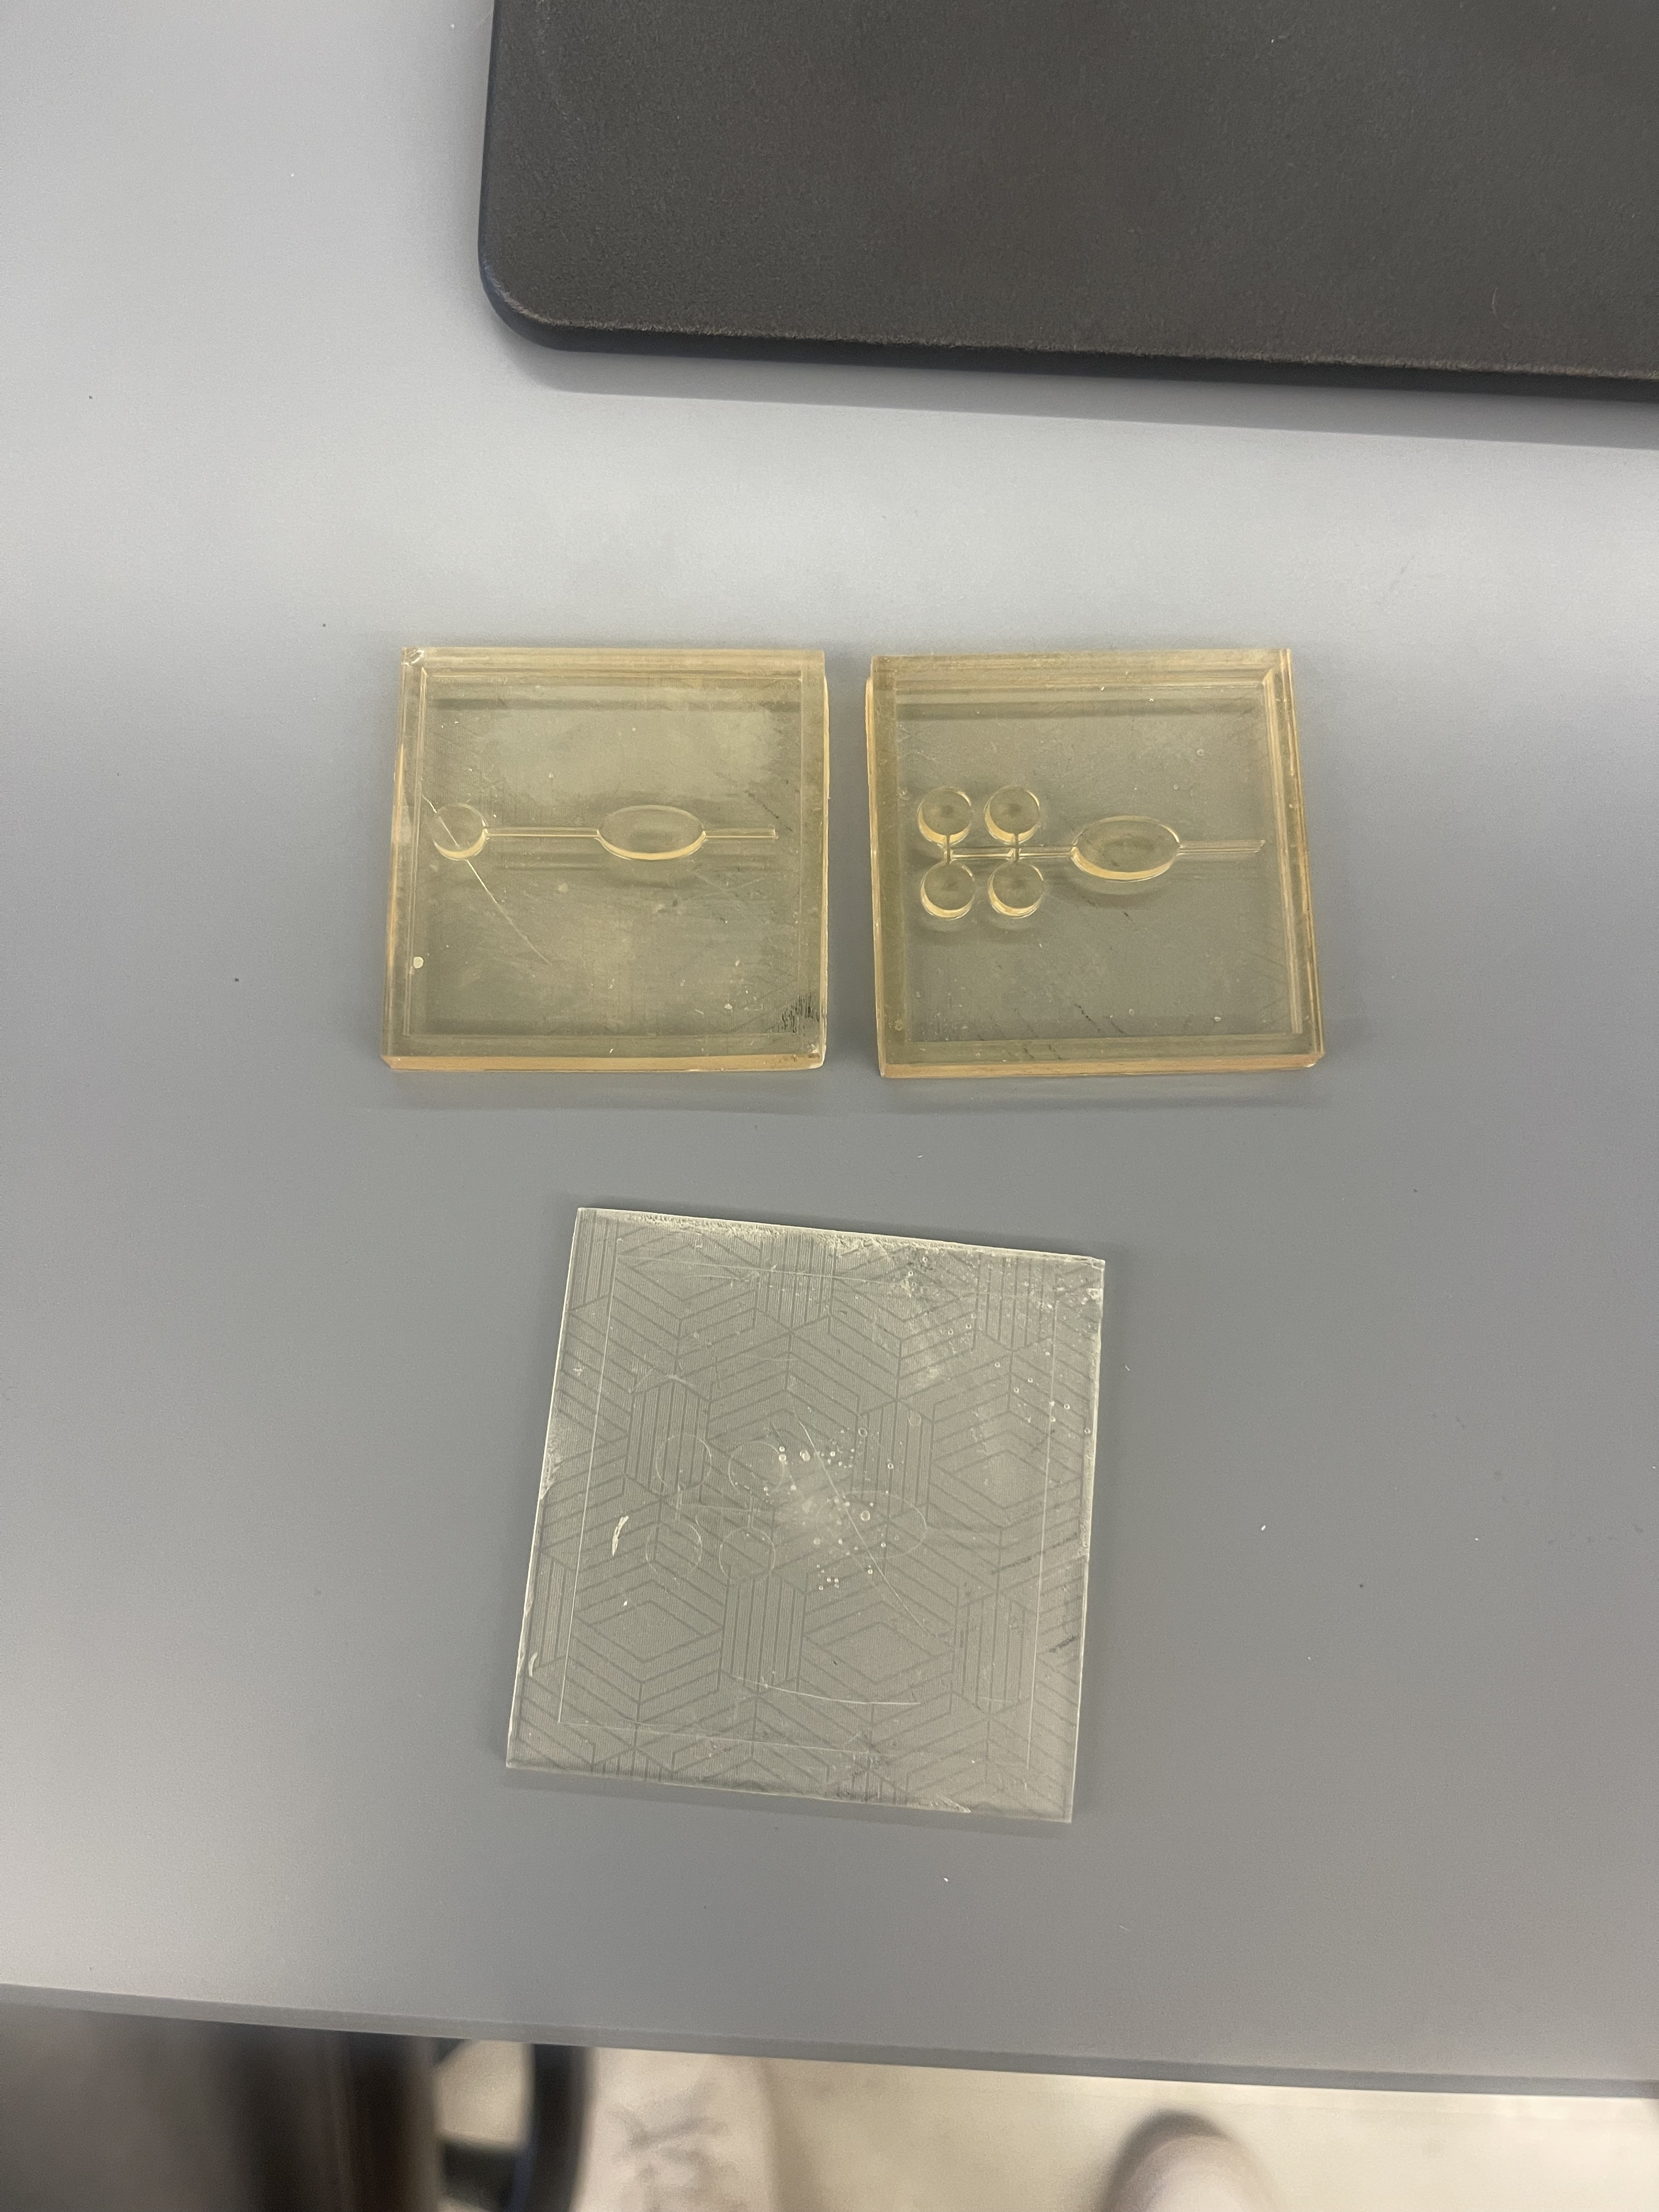
\includegraphics[width=0.45\linewidth]{fig13.jpg}
    \caption{3D printed microfluidic patch molds}
    \label{fig13}
\end{figure}

\begin{figure}[H]
    \centering
    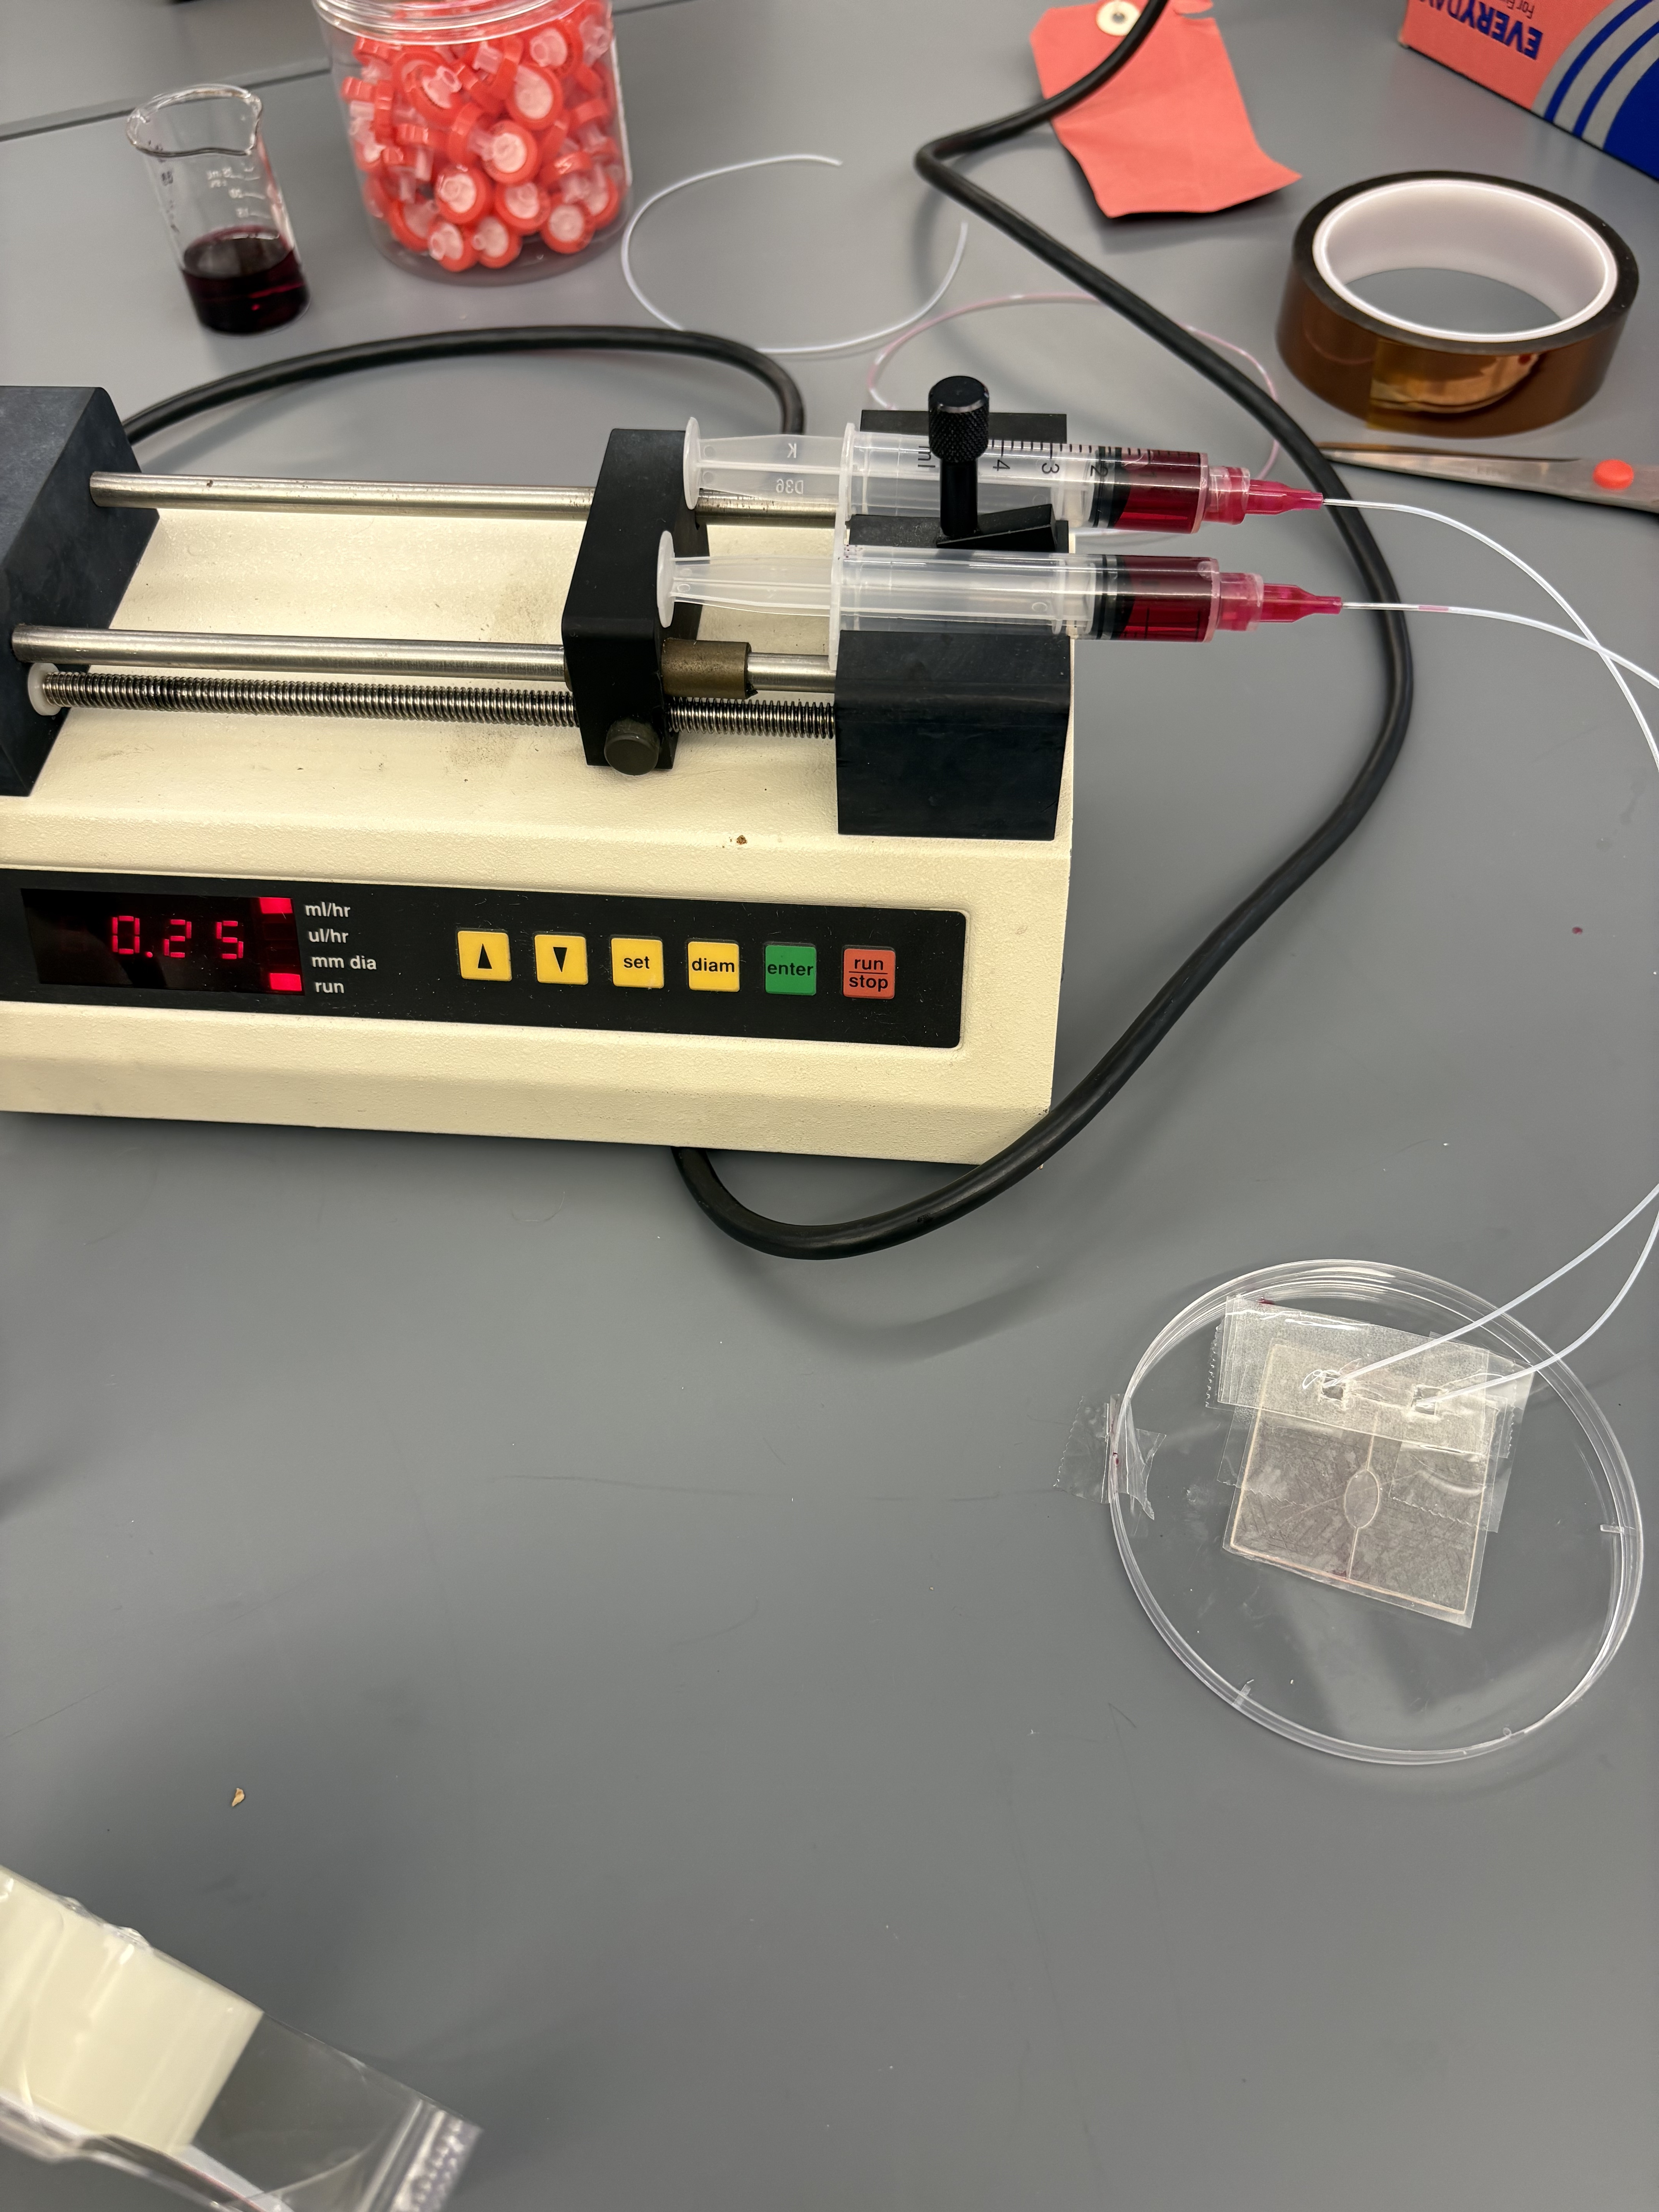
\includegraphics[width=0.45\linewidth]{fig14.jpg}
    \caption{Syringe pump testing set up with the dual-inlet printed chip}
    \label{fig14}
\end{figure}

\bigskip

\section{Results}

\smallskip

\subsection{Device}
The diffuse scatter shown in Fig.\ref{fig19} indicates that the potentiostat is operating outside it's linear region. Under such conditions, some measurements obscured the paired anodic and cathodic peaks of the ideal CV characteristics. It is derived that the residual ripples usually in tens of millivolts of voltage ramp is comparable to potentials that trigger redox reactions. Resultantly, the electrochemical peaks appear as random distribution along the current axis. 


\begin{figure}[H]
    \centering
    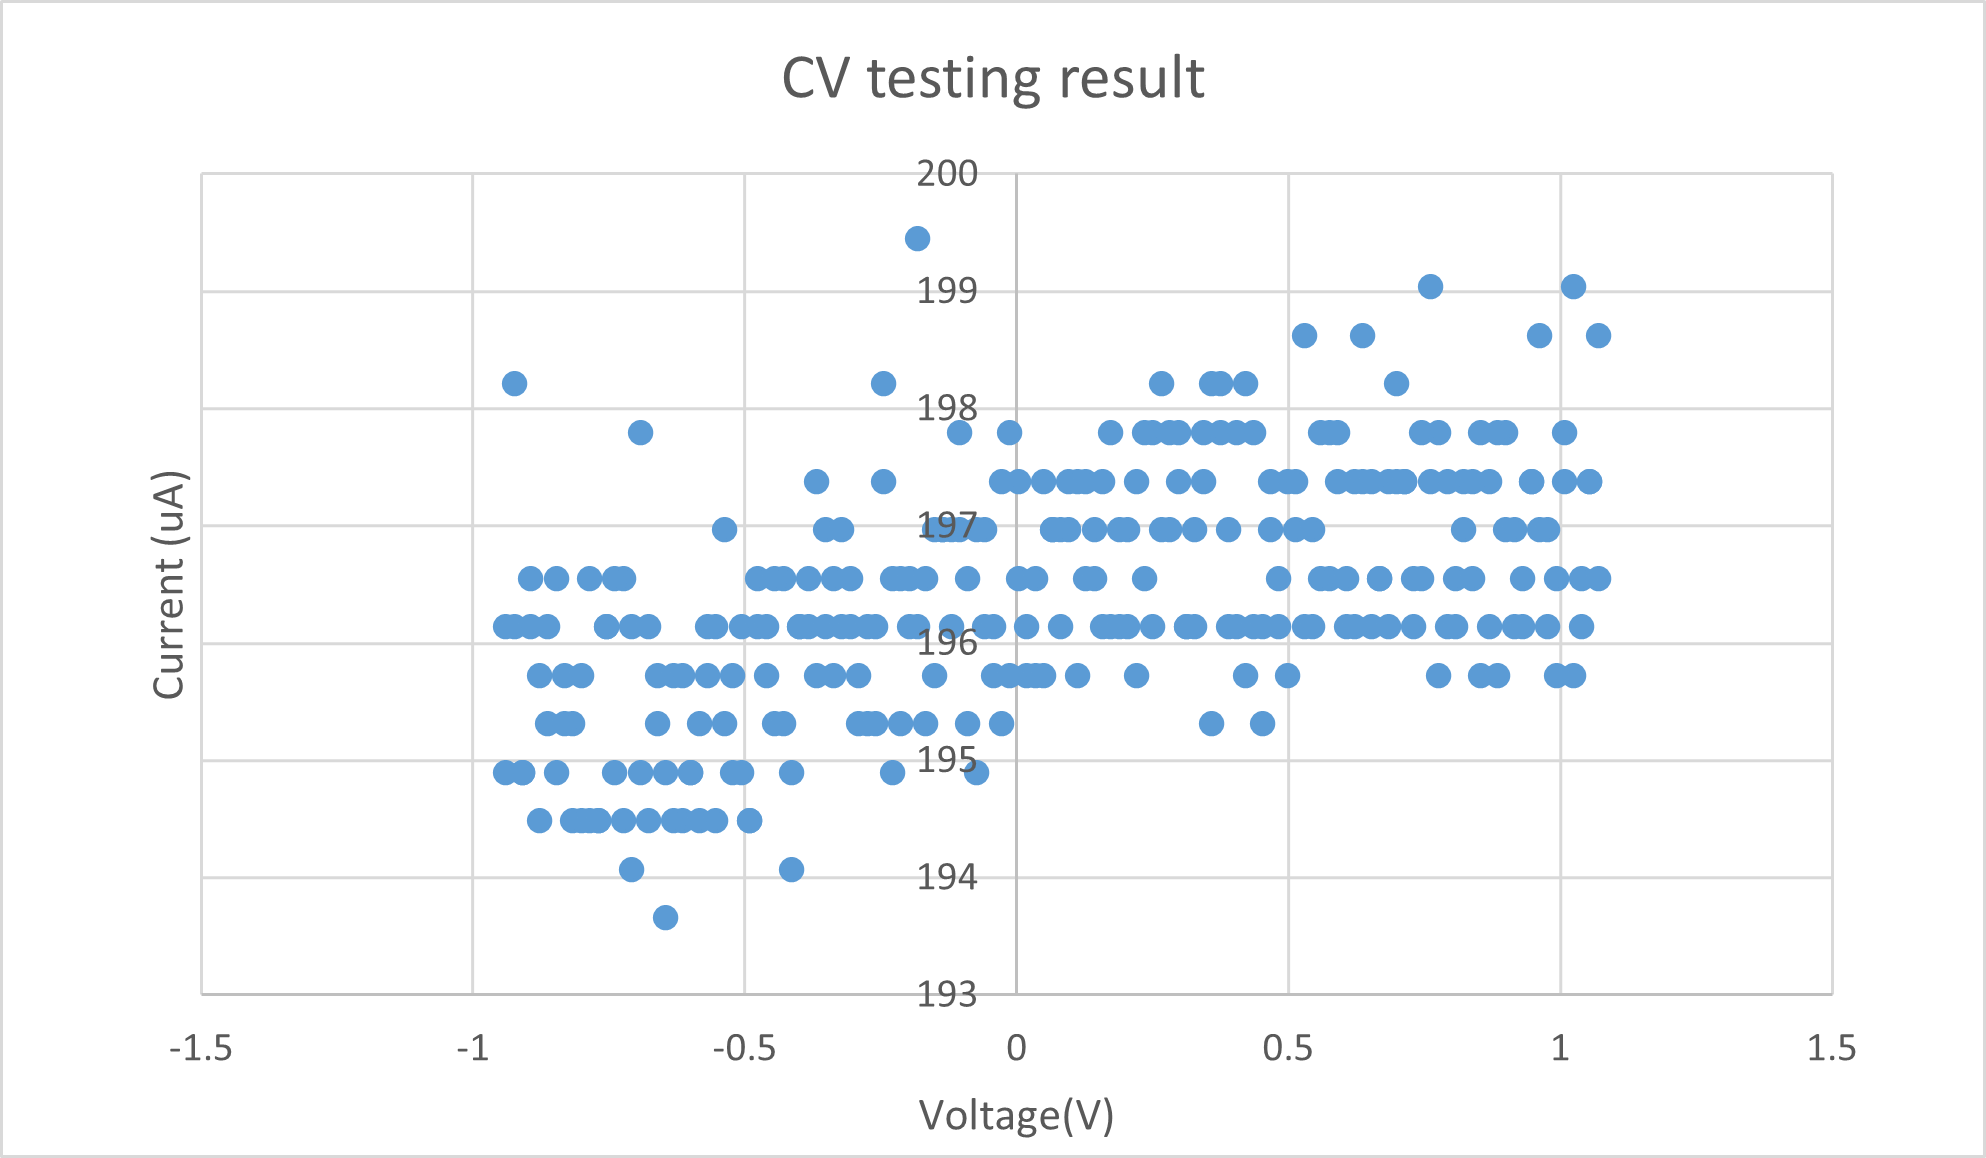
\includegraphics[width=\linewidth]{fig19.png}
    \caption{CV of proposed potentiostat circuit}
    \label{fig19}
\end{figure}


As an alternative, the LMP91000 from Texas Instrument is a integrated, low-power potentiostat front end for electrochemical applications. It incorporates programmable transimpedance amplifier, bias generator and gain network and configures via an I\textsuperscript{2}C interface without swapping components. We attempted to benchmark the LMP91000EVM against our prototype with elements of the experimental workflow being preserved. We employed a three-lead electrochemical sensor Metrohm 110 in 0.1M PBS, the same Arduino Uno R3 for power supply and data processing (Fig.\ref{fig21}). Configuration was written via Arduino IDE (Appendix.\ref{LMP91000EVM}). Within the LMP91000EVM, the transimpedance gain resistor $R_{TIA}$ and load resistor $R_{load}$ is set to $35k\,\Omega$ and $10\,\Omega$ respectively, reference source is set to external with internal zero is set to 50\% of the reference voltage. And hence by varying the bias percentage (\textpm24\%), we would be able to maintain potential sweep between working and reference electrodes ($V_{WE} \;-V_{RE}$). 

\begin{figure}[H]
    \centering
    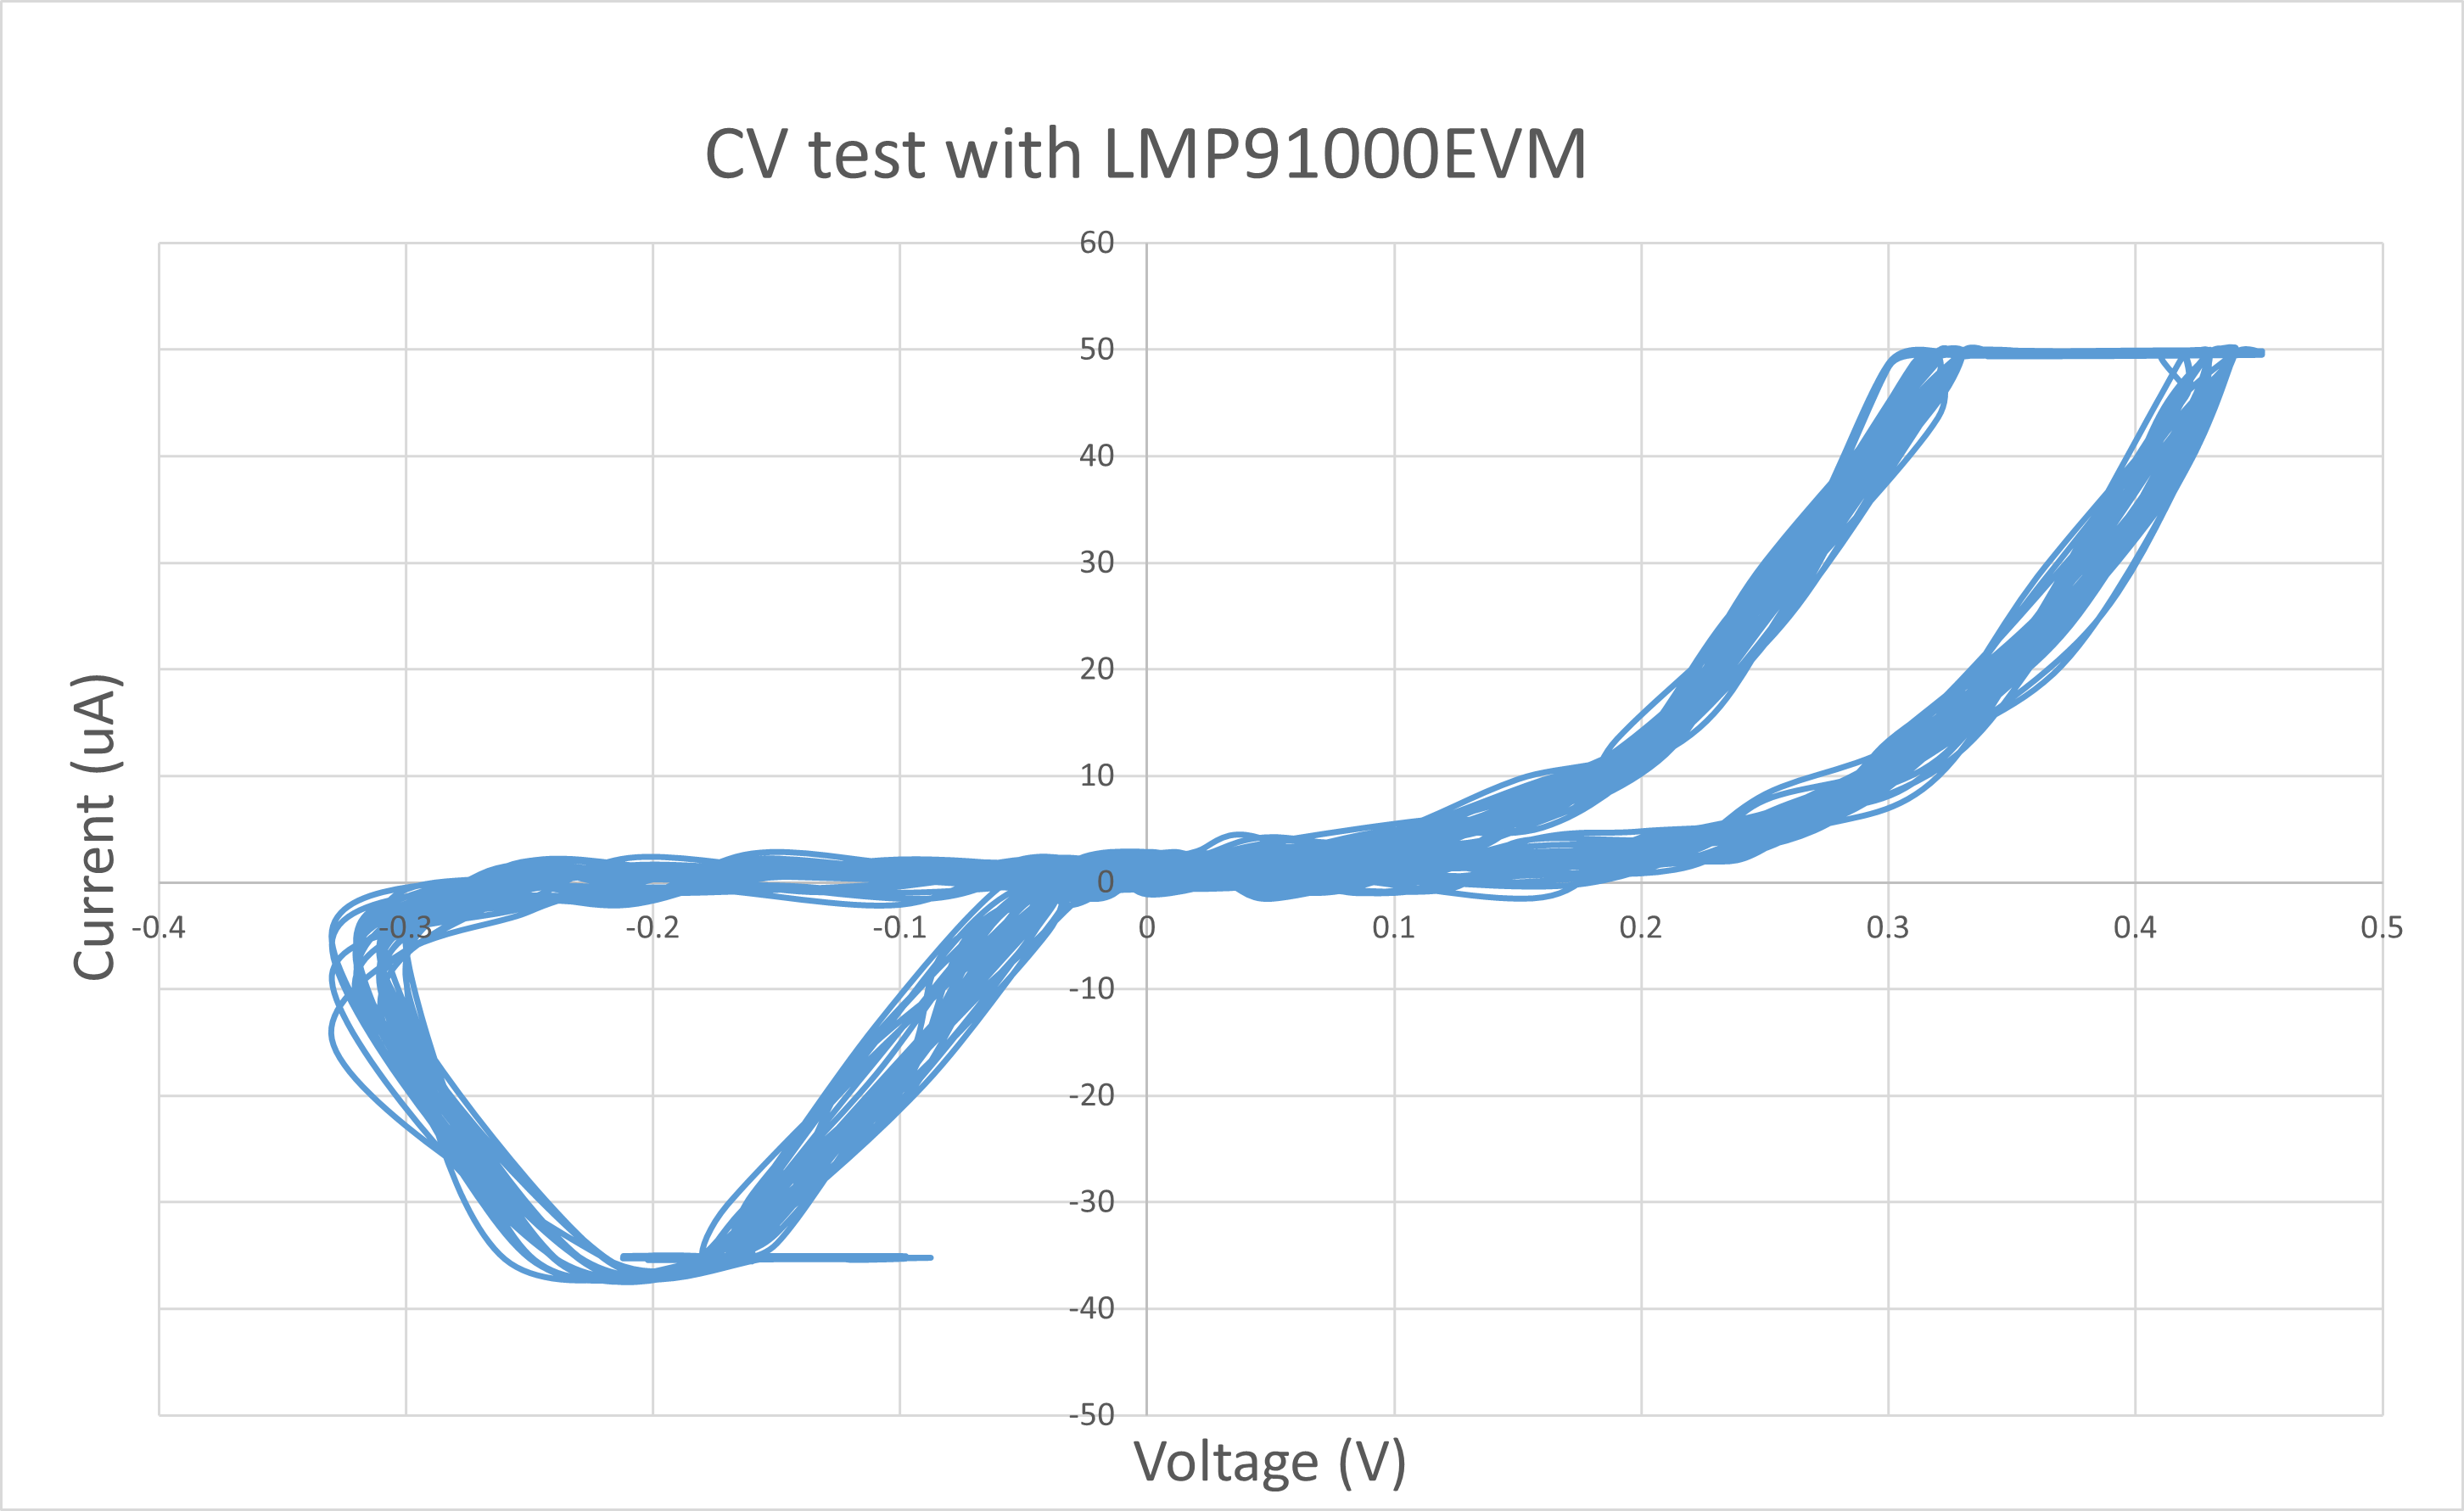
\includegraphics[width=\linewidth]{fig20.png}
    \caption{CV results with LMP91000EVM}
    \label{fig}
\end{figure}

The resulting CV test clearly exhibits both anodic and cathodic peaks at $+300\text{---}400\,\mathrm{mV}$ and $-200\,\mathrm{mV}$ respectively, with peak currents of \text 49$\mu\text A$ and \text -35$\mu\text A$. The immediate improvements confirm that the LMP91000EVM delivers analytical accuracy and stability while it can also shrink the footprint if with LMP91000. 


\subsection{Sensor}
In the CV results for sensor 1, small peaks are visible, however there are two negative peaks, indicating there was some mixing of the silver ink.

\smallskip
\begin{figure}[H]
    \centering
    
\includegraphics[width=0.45\linewidth]{images/fig16.png}
    \caption{CV of Screen-printed sensor}
    \label{fig}
\end{figure}
\smallskip

In the prussian blue deposition CV for the inkjet printed sensor, the peaks are almost non-existent and hard to see. A successful PB deposition would have one oxidation and one reduction peak both increasing over time as the PB is deposited.

\smallskip
\begin{figure}[H]
    \centering
    
\includegraphics[width=0.45\linewidth]{images/fig17.png}
    \caption{CV of PB deposition, inkjet printer}
    \label{fig}
\end{figure}
\smallskip

\subsection{Microfluidics}
Three iterative designs of the microfluidic patch were tested using SimScale CFD simulations (include parameters). In the preliminary layout, the design included four 1.5mm radius inlets, a 15mm x 300µm x 300µm channel, and a 31mm x 5.6mm reservoir to house the sensor. Simulations indicated that old sweat would accumulate in the reservoir's corners, as the expected velocity of sweat in the corners was very slow compared to sweat closer to the center of the reservoir. Additionally, sweat flow across the reservoir required approximately six minutes, making the design unsuitable for this project. The second design featured a modified 11mm x 6mm elliptical reservoir to accommodate the updated sensor layout, as well as a single inlet to prevent bubble formation. While sweat accumulation was prevented, flow time increased to nine minutes, and expanding the inlet size did not improve flow rate. The third design implemented the reservoir from design two, but reverted to the original four-inlet layout to speed up the flow rate. In this design, sweat did not accumulate and took roughly 2 minutes to cross the reservoir, suggesting that it may be suitable for our project.
The initial attempt to fabricate the microfluidic patch using PDMS was unsuccessful. Despite heating the molds for three hours at 70°C, the cured PDMS could not be extracted from the molds without breaking apart. The second attempt, where the microfluidic patch was 3D printed, was partially successful. Many prints were unusable due to low resolution. However, high resolution prints of single and dual inlet designs were achieved. These were tested using the previously mentioned syringe pump testing protocol. Data was plotted and compared with target metrics, as seen in figure x. The data indicates that the single inlet design flow rate is far too slow, as expected. It also shows that the dual inlet design is much closer to the target speed. Further, no bubbles were observed during the single inlet test, but some bubbles were present in the early stages of the dual inlet test.


\begin{figure}[hptb]
    \centering
    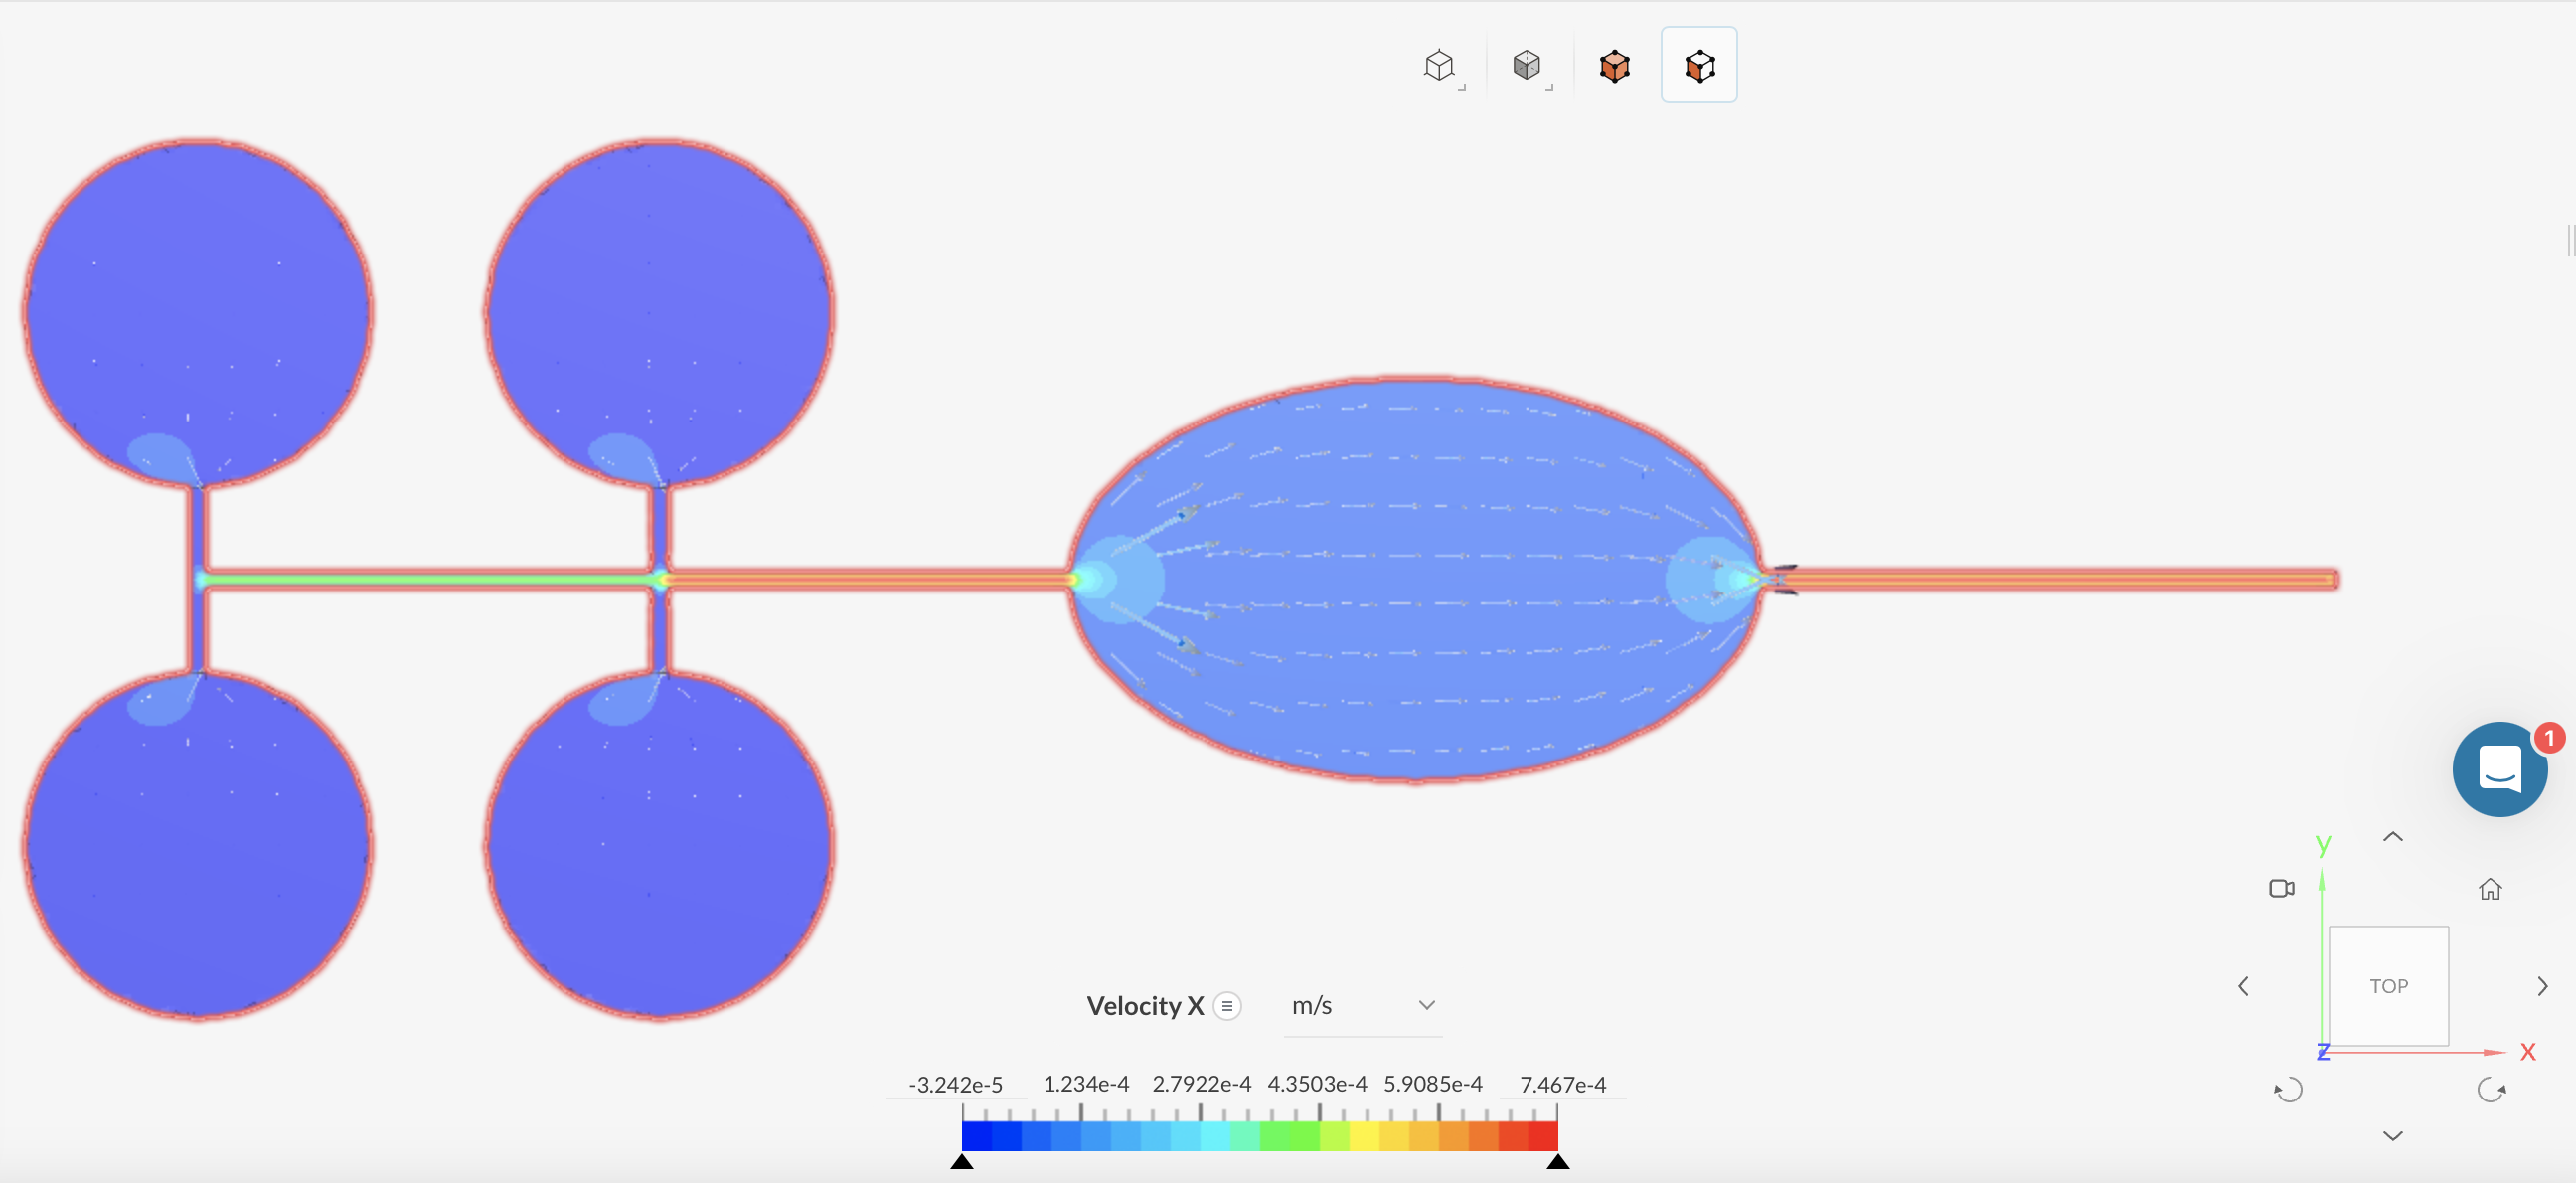
\includegraphics[width=0.45\linewidth]{fig10.png}
    \caption{Microfluidic Patch Design 3 Layout and CFD Simulation Results}
    \label{fig}
\end{figure}

\begin{figure}[hptb]
    \centering
    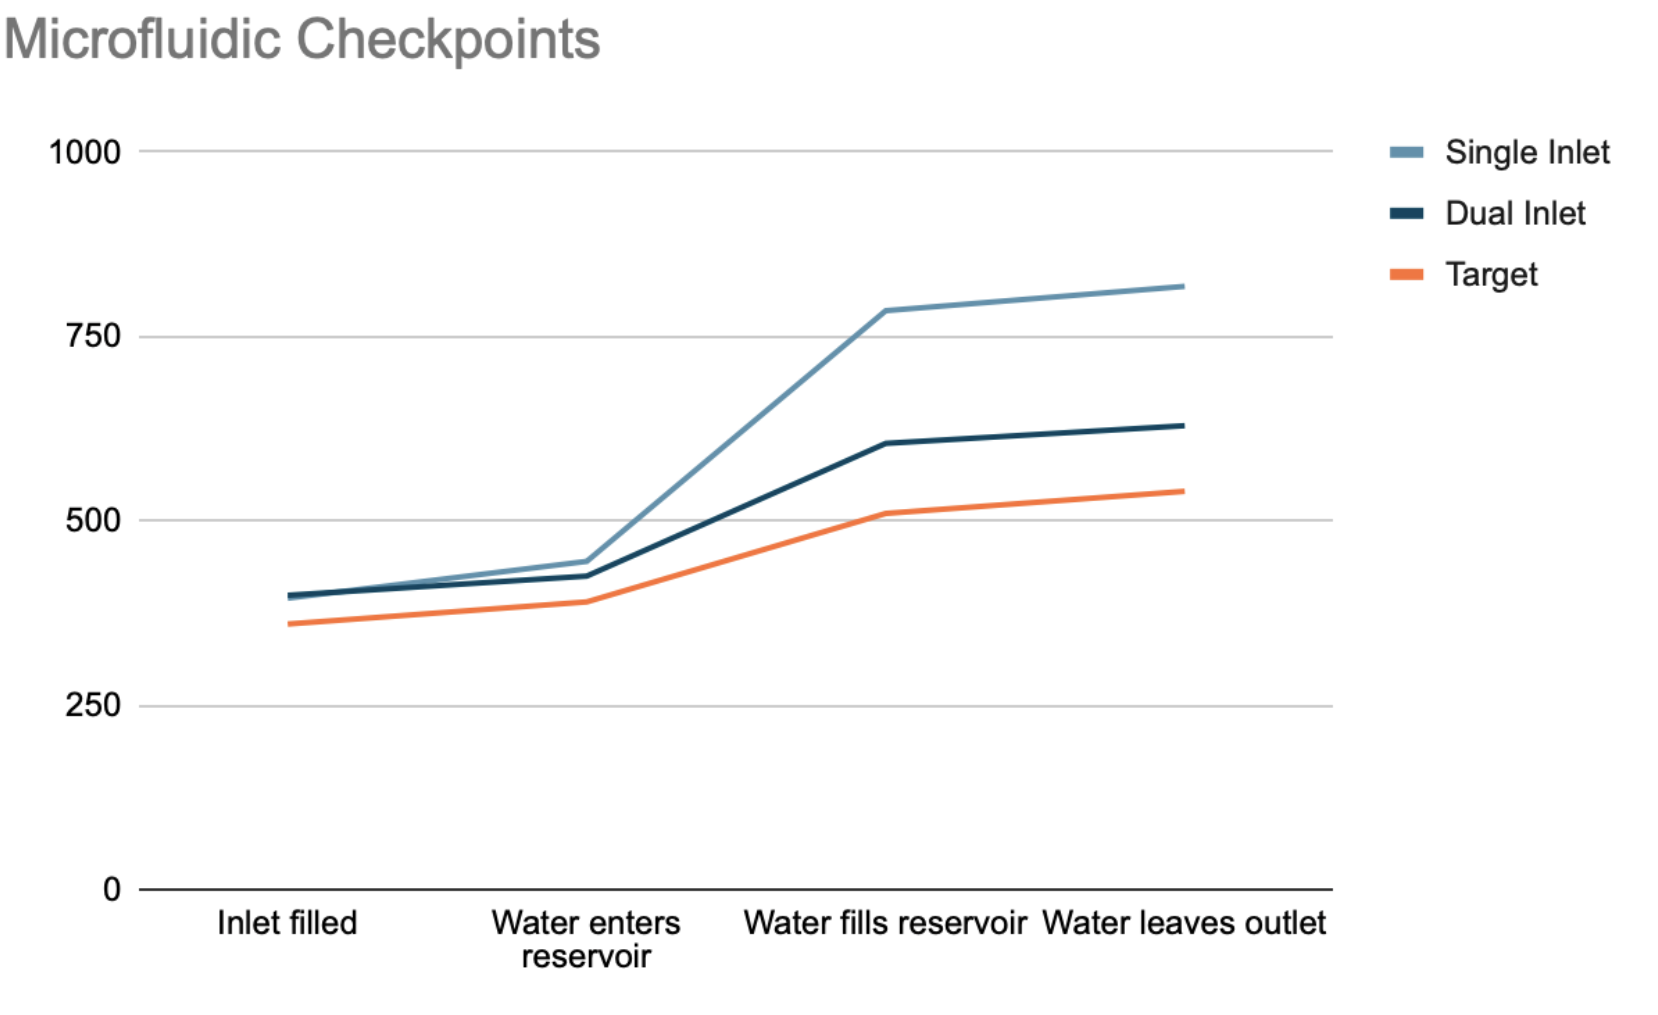
\includegraphics[width=0.5\linewidth]{fig15.png}
    \caption{Syringe pump simulation results for single and dual inlet designs}
    \label{fig}
\end{figure}

\bigskip

\section{Discussion}
We first implement a discrete, driven by PWM potentiostat prototype and conduct CV testing with Arduino Uno R3 board. While we verified its basic functionality in simulation, it's rail limitations and component tolerances produced high noise and obscured the expected redox peaks from CV test. We then replaced the prototype with the LMP91000EVM and greatly improved current stability and accuracy with clean anodic and cathodic responses. Having validated the single-chip front end, our next step is to integrate the LMP91000 with nRF52832 module to evaluate the full wearable prototype. 

In the CV testing it can be seen that there is contamination of the carbon signal with silver, shown by the two peaks instead of one in the graphs. Next steps to correct this is to apply the isolation solution more generously to all the silver parts of the sensor to ensure that there is no contamination. Once ideal CV graphs have been obtained, the working electrodes can then be modified with their respective enzymes and tested again. 
In prussian blue deposition on the working electrodes of the inkjet-printed sensor, the PB solution most likely came in contact with the silver of the reference electrode, leading to a contamination of the results. To correct this, the sensor design will be modified to make it larger and add more space between the electrodes. The separation will allow for a more accurate deposition of PB without contamination from the silver of the reference electrode.


For the microfluidic patch, the team determined that an elliptical reservoir was crucial for avoiding sweat build up. It was also noted that more than one inlet was necessary to achieve the required speed across the reservoir. However, using more than one inlet presents the challenge of dealing with bubbles in the channel, which can impact measurements. A potential solution for this would be to add very small holes in the top of the inlets to allow air to escape. Additionally, while the team was able to validate designs using 3D printed patches, a new method of manufacturing a flexible and biocompatible patch will need to be formulated.
\bigskip

\section{Acknowledgments} 

Thank you to Dr Moreto, Dr Sempionatto, Beatriz Mayol, and Julieta Nava Granados for their guidance and assistance during this project.

\bigskip



\section{References}
[1] E. C. Lee, M. S. Fragala, S. A. Kavouras, R. M. Queen, J. L. Pryor, and D. J. Casa, “Biomarkers in Sports and Exercise: Tracking Health, Performance, and Recovery in Athletes,” Journal of strength and conditioning research, vol. 31, no. 10, pp. 2920–2937, 2017, doi: https://doi.org/10.1519/JSC.0000000000002122.

[2]  T. Huang, Z. Liang, K. Wang, X. Miao, and L. Zheng, “Novel insights into athlete physical recovery concerning lactate metabolism, lactate clearance and fatigue monitoring: A comprehensive review,” Frontiers in Physiology, vol. 16, Mar. 2025, doi: https://doi.org/10.3389/fphys.2025.1459717.

[3] M. Flockhart and F. J. Larsen, “Continuous Glucose Monitoring in Endurance Athletes: Interpretation and Relevance of Measurements for Improving Performance and Health,” Sports Medicine, vol. 54, Sep. 2023, doi: https://doi.org/10.1007/s40279-023-01910-4.

[4] Y. Xiao et al., “Noninvasive glucose monitoring using portable GOx-Based biosensing system,” Analytica Chimica Acta, vol. 1287, p. 342068, Nov. 2023, doi: https://doi.org/10.1016/j.aca.2023.342068.

‌[5] D. Grieshaber, R. MacKenzie, J. Vörös, and E. Reimhult, “Electrochemical Biosensors - Sensor Principles and Architectures,” Sensors, vol. 8, no. 3, pp. 1400–1458, Mar. 2008, doi: https://doi.org/10.3390/s80314000.


[6] J. R. Camargo et al., “Development of conductive inks for electrochemical sensors and biosensors,” Microchemical Journal, vol. 164, p. 105998, May 2021, doi: https://doi.org/10.1016/j.microc.2021.105998.

[7] A. Kangmennaa, Richard Baffour Forkuo, and Eric Selorm Agorku, “Carbon-based electrode materials for sensor application: a review,” Sensing Technology, vol. 2, no. 1, May 2024, doi: https://doi.org/10.1080/28361466.2024.2350174.

[8] F. Poletti et al., “Continuous capillary-flow sensing of glucose and lactate in sweat with an electrochemical sensor based on functionalized graphene oxide,” Sensors and Actuators B: Chemical, vol. 344, pp. 130253–130253, Oct. 2021, doi: https://doi.org/10.1016/j.snb.2021.130253.

[9] Apinya Obma et al., “Measurement of sweat lactate levels in exercise and non-exercise activities using capillary electrophoresis system with contactless conductivity detection and cyclodextrin-modified buffer,” Arabian Journal of Chemistry, vol. 16, no. 11, pp. 105255–105255, Sep. 2023, doi: https://doi.org/10.1016/j.arabjc.2023.105255.

[10] Y. Yin, Z. Tan, W. Zhu, Z. Pu, H. Yu, R. Wang, and D. Li, "A wearable microfluidic system for efficient sweat collection and real-time detection," Talanta, vol. 274, p. 125967, 2024. [Online]. Available: https://doi.org/10.1016/j.talanta.2024.125967.

[11] J. Min et al., “An autonomous wearable biosensor powered by a perovskite solar cell,” Nature Electronics, vol. 6, no. 8, pp. 630–641, 2023.

[12] A. V. Subbarayalu et al., “Lactate threshold training to improve long-distance running performance: A narrative review,” Montenegrin Journal of Sports Science and Medicine, vol. 20, pp. 3–13, 2024, doi: 10.26773/mjssm.240303.



‌









\clearpage            
\onecolumn            % switch to one column
\appendices


\section{}
The following sensor configurations have been used for design and testing using the Inkscape software. The working electrodes (WE), reference electrode (RE), counter electrode (CE), and relevant dimensions have been labeled.
\smallskip
\begin{figure}[H]
    \centering
    
\includegraphics[width=0.45\linewidth]{images/fig18.png}
    \caption{Manual Screen Printed Design}
    \label{fig}
\end{figure}
\smallskip
The carbon ink used for manual screen printing is a conductive ink from Creative Materials, further information can be found in the datasheet \url{https://server.creativematerials.com/datasheets/DS_126_48.pdf}. The silver ink used for manual screen printing is a medical grade electrically conductive ink from Creative Materials, further information can be found in the datasheet \url{https://server.creativematerials.com/datasheets/DS_124_36.pdf}.

\smallskip
\begin{figure}[H]
    \centering
    
\includegraphics[width=0.45\linewidth]{images/fig19.png}
    \caption{Inkjet Printed Design}
    \label{fig}
\end{figure}

\smallskip
\begin{figure}[H]
    \centering
    
\includegraphics[width=0.45\linewidth]{images/fig20.png}
    \caption{Tentative Final Design}
    \label{fig}
\end{figure}
\smallskip
In the final design of the sensor, the ideal dimensions will be about half the size of those currently being used to test the sensor.

\section{}
The Styrene Ethylene Butylene Styrene (SEBS) isolation solution was prepared using nine parts of SEBS pellets to one part of liquid tetrahydrofuran (THF). The SEBS was dissolved in the THF by placing the mixture in an ultrasonic bath for 30 minutes or until dissolved. Once the solution was complete, it was pipetted onto the surface sensor on the silver part of the electrode from the carbon connection point up to the connector pads as shown in the image. 
The solution was placed to cover the majority of electrode, leaving the leads uncovered, as per the image below.
\smallskip
\begin{figure}[H]
    \centering
    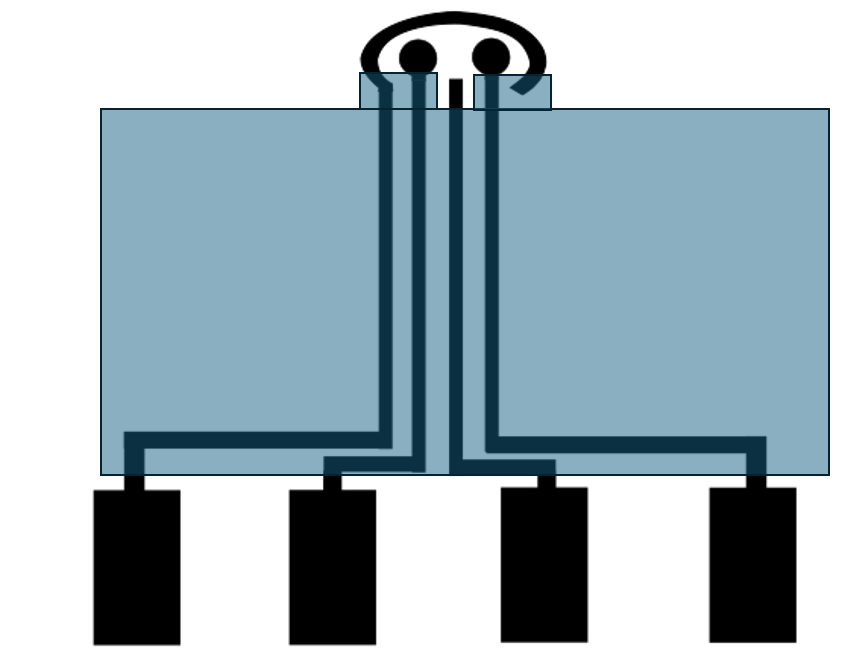
\includegraphics[width=0.45\linewidth]{images/fig21.png}
    \caption{SEBS solution placement on sensor}
    \label{fig}
\end{figure}
\smallskip

\section{}

\begin{figure}[H]
    \centering
    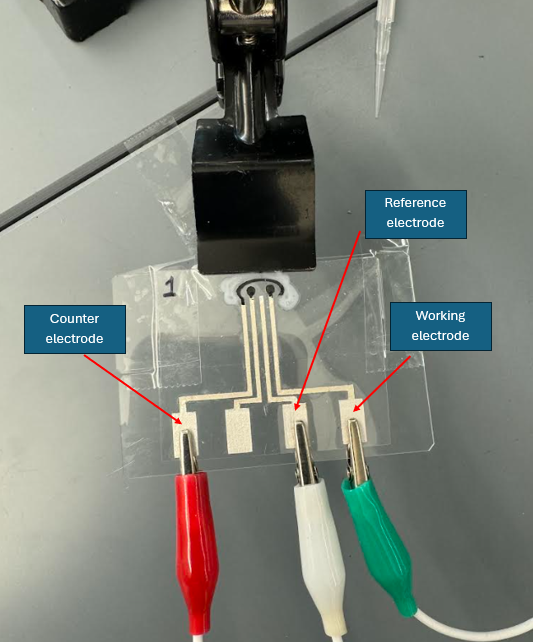
\includegraphics[width=0.45\linewidth]{images/fig22.png}
    \caption{CV setup of manual screen printed sensor}
    \label{fig}
\end{figure}
\smallskip

\begin{figure}[H]
    \centering
    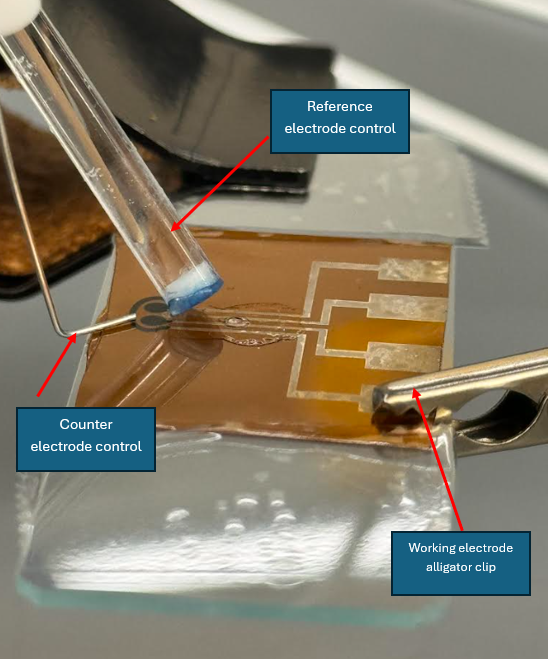
\includegraphics[width=0.45\linewidth]{images/fig23.png}
    \caption{Prussian Blue deposition on inkjet printed sensor CV setup}
    \label{fig}
\end{figure}
\smallskip

\section{}

\begin{figure}[H]
    \centering
    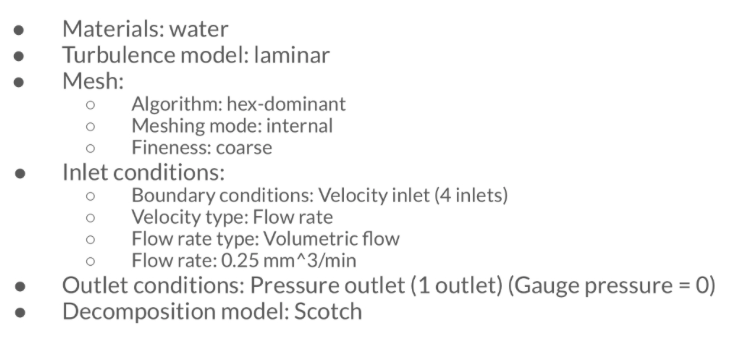
\includegraphics[width=0.9\linewidth]{images/fig24.png}
    \caption{SimScale Input Parameters for Microfluidics Testing}
    \label{fig}
\end{figure}
\smallskip

\section{Circuitry Schematics}
\begin{figure}[H]
    \centering
    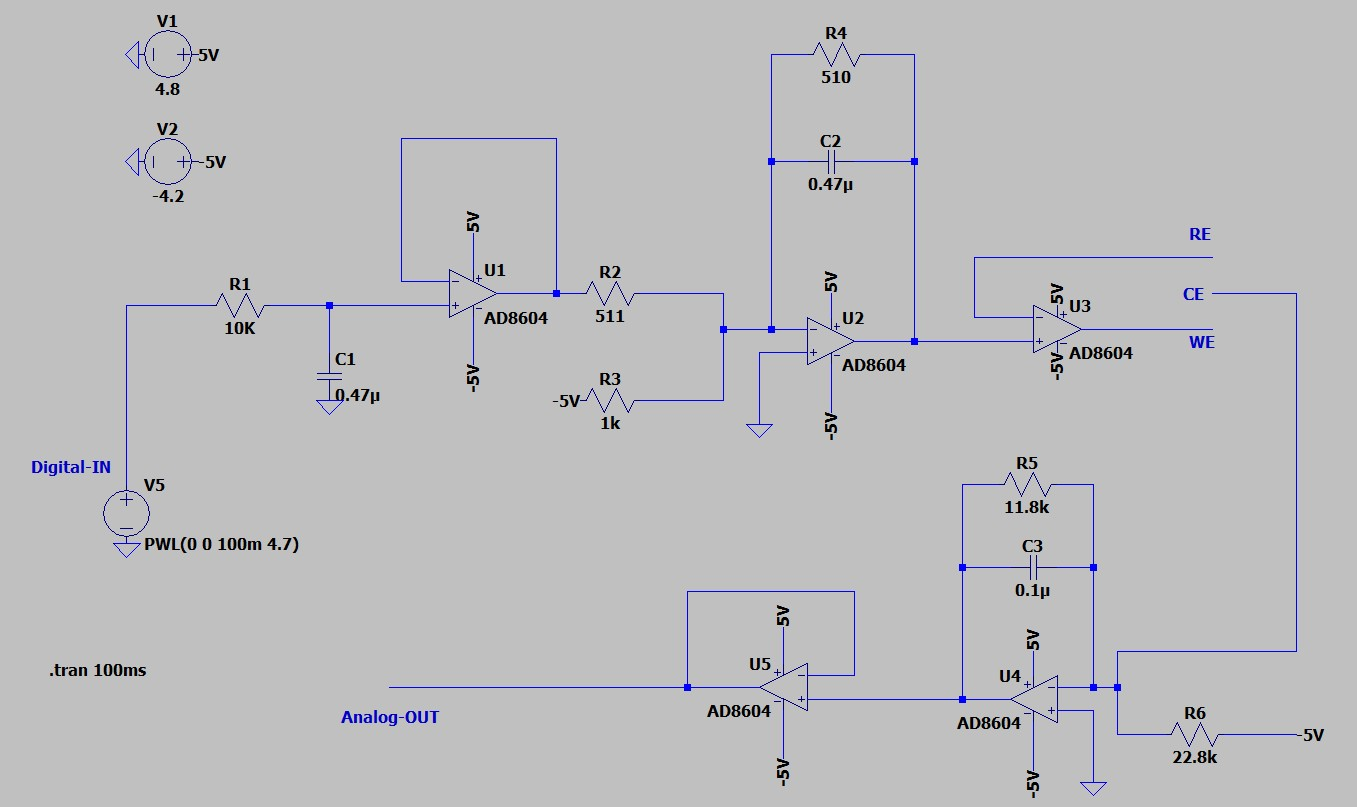
\includegraphics[width=\linewidth]{fig1.jpg}
    \caption{Full schematic design of the potentiostat in LTspice}
    \label{fig1}
\end{figure}

\begin{figure}[H]
    \centering
    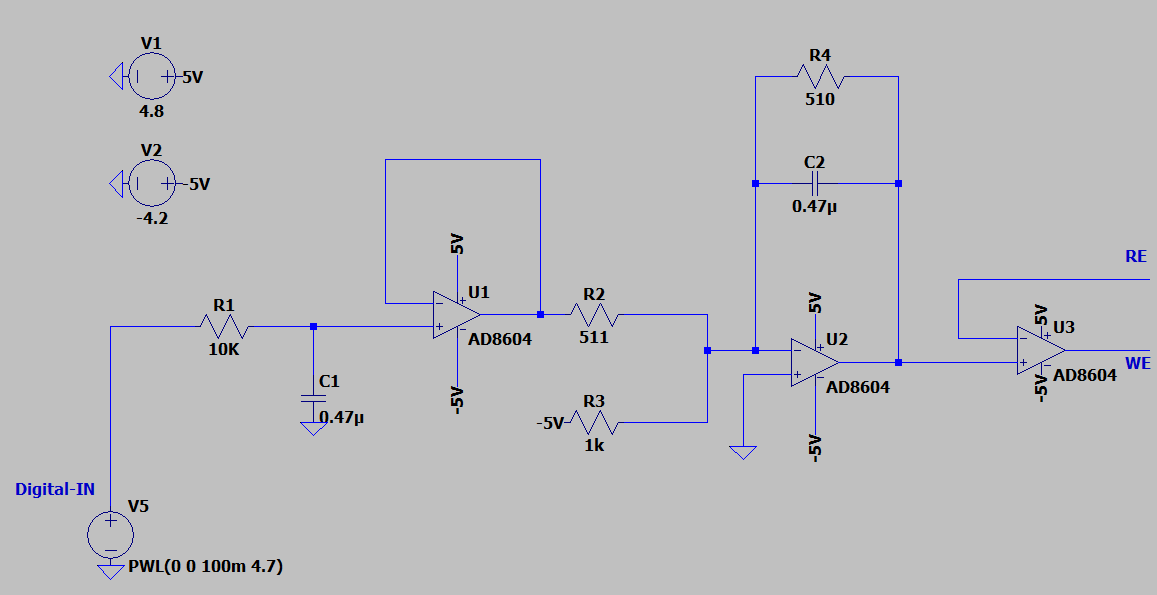
\includegraphics[width=\linewidth]{fig16.png}
    \caption{Schematic of excitation chain}
    \label{fig16}
\end{figure}

\begin{figure}[H]
    \centering
    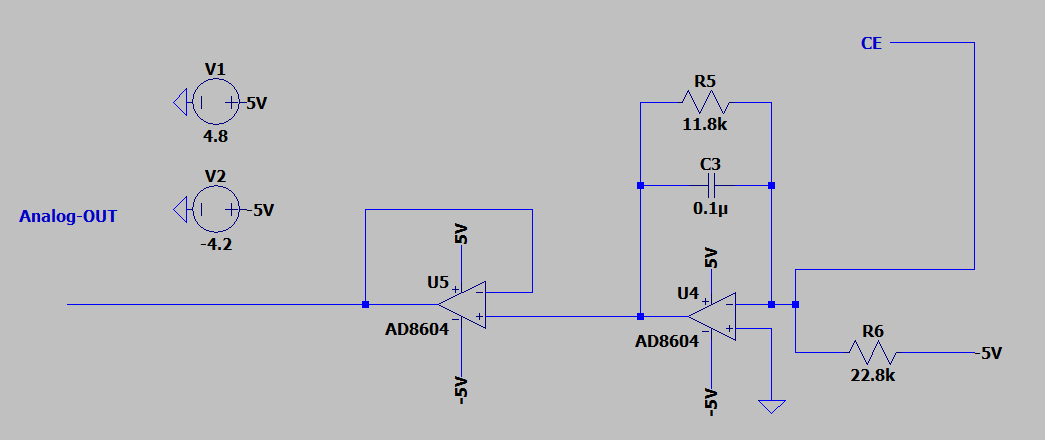
\includegraphics[width=\linewidth]{fig17.png}
    \caption{Schematic of acquisition chain}
    \label{fig17}
\end{figure}

\section{Hardware assembly}

\begin{figure}[H]
    \centering
    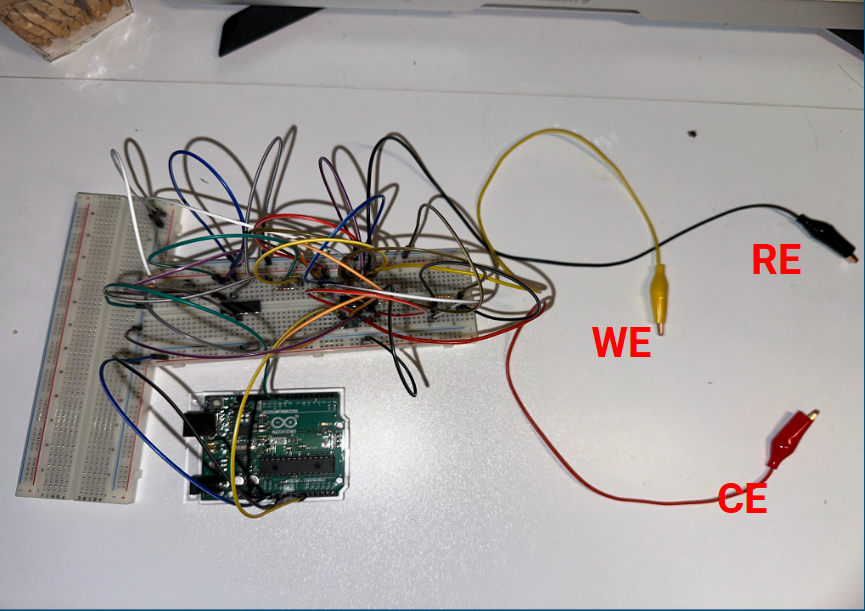
\includegraphics[width=\linewidth]{fig18.png}
    \caption{Potentiostat hardware assembly}
    \label{fig18}
\end{figure}

\begin{figure}[H]
    \centering
    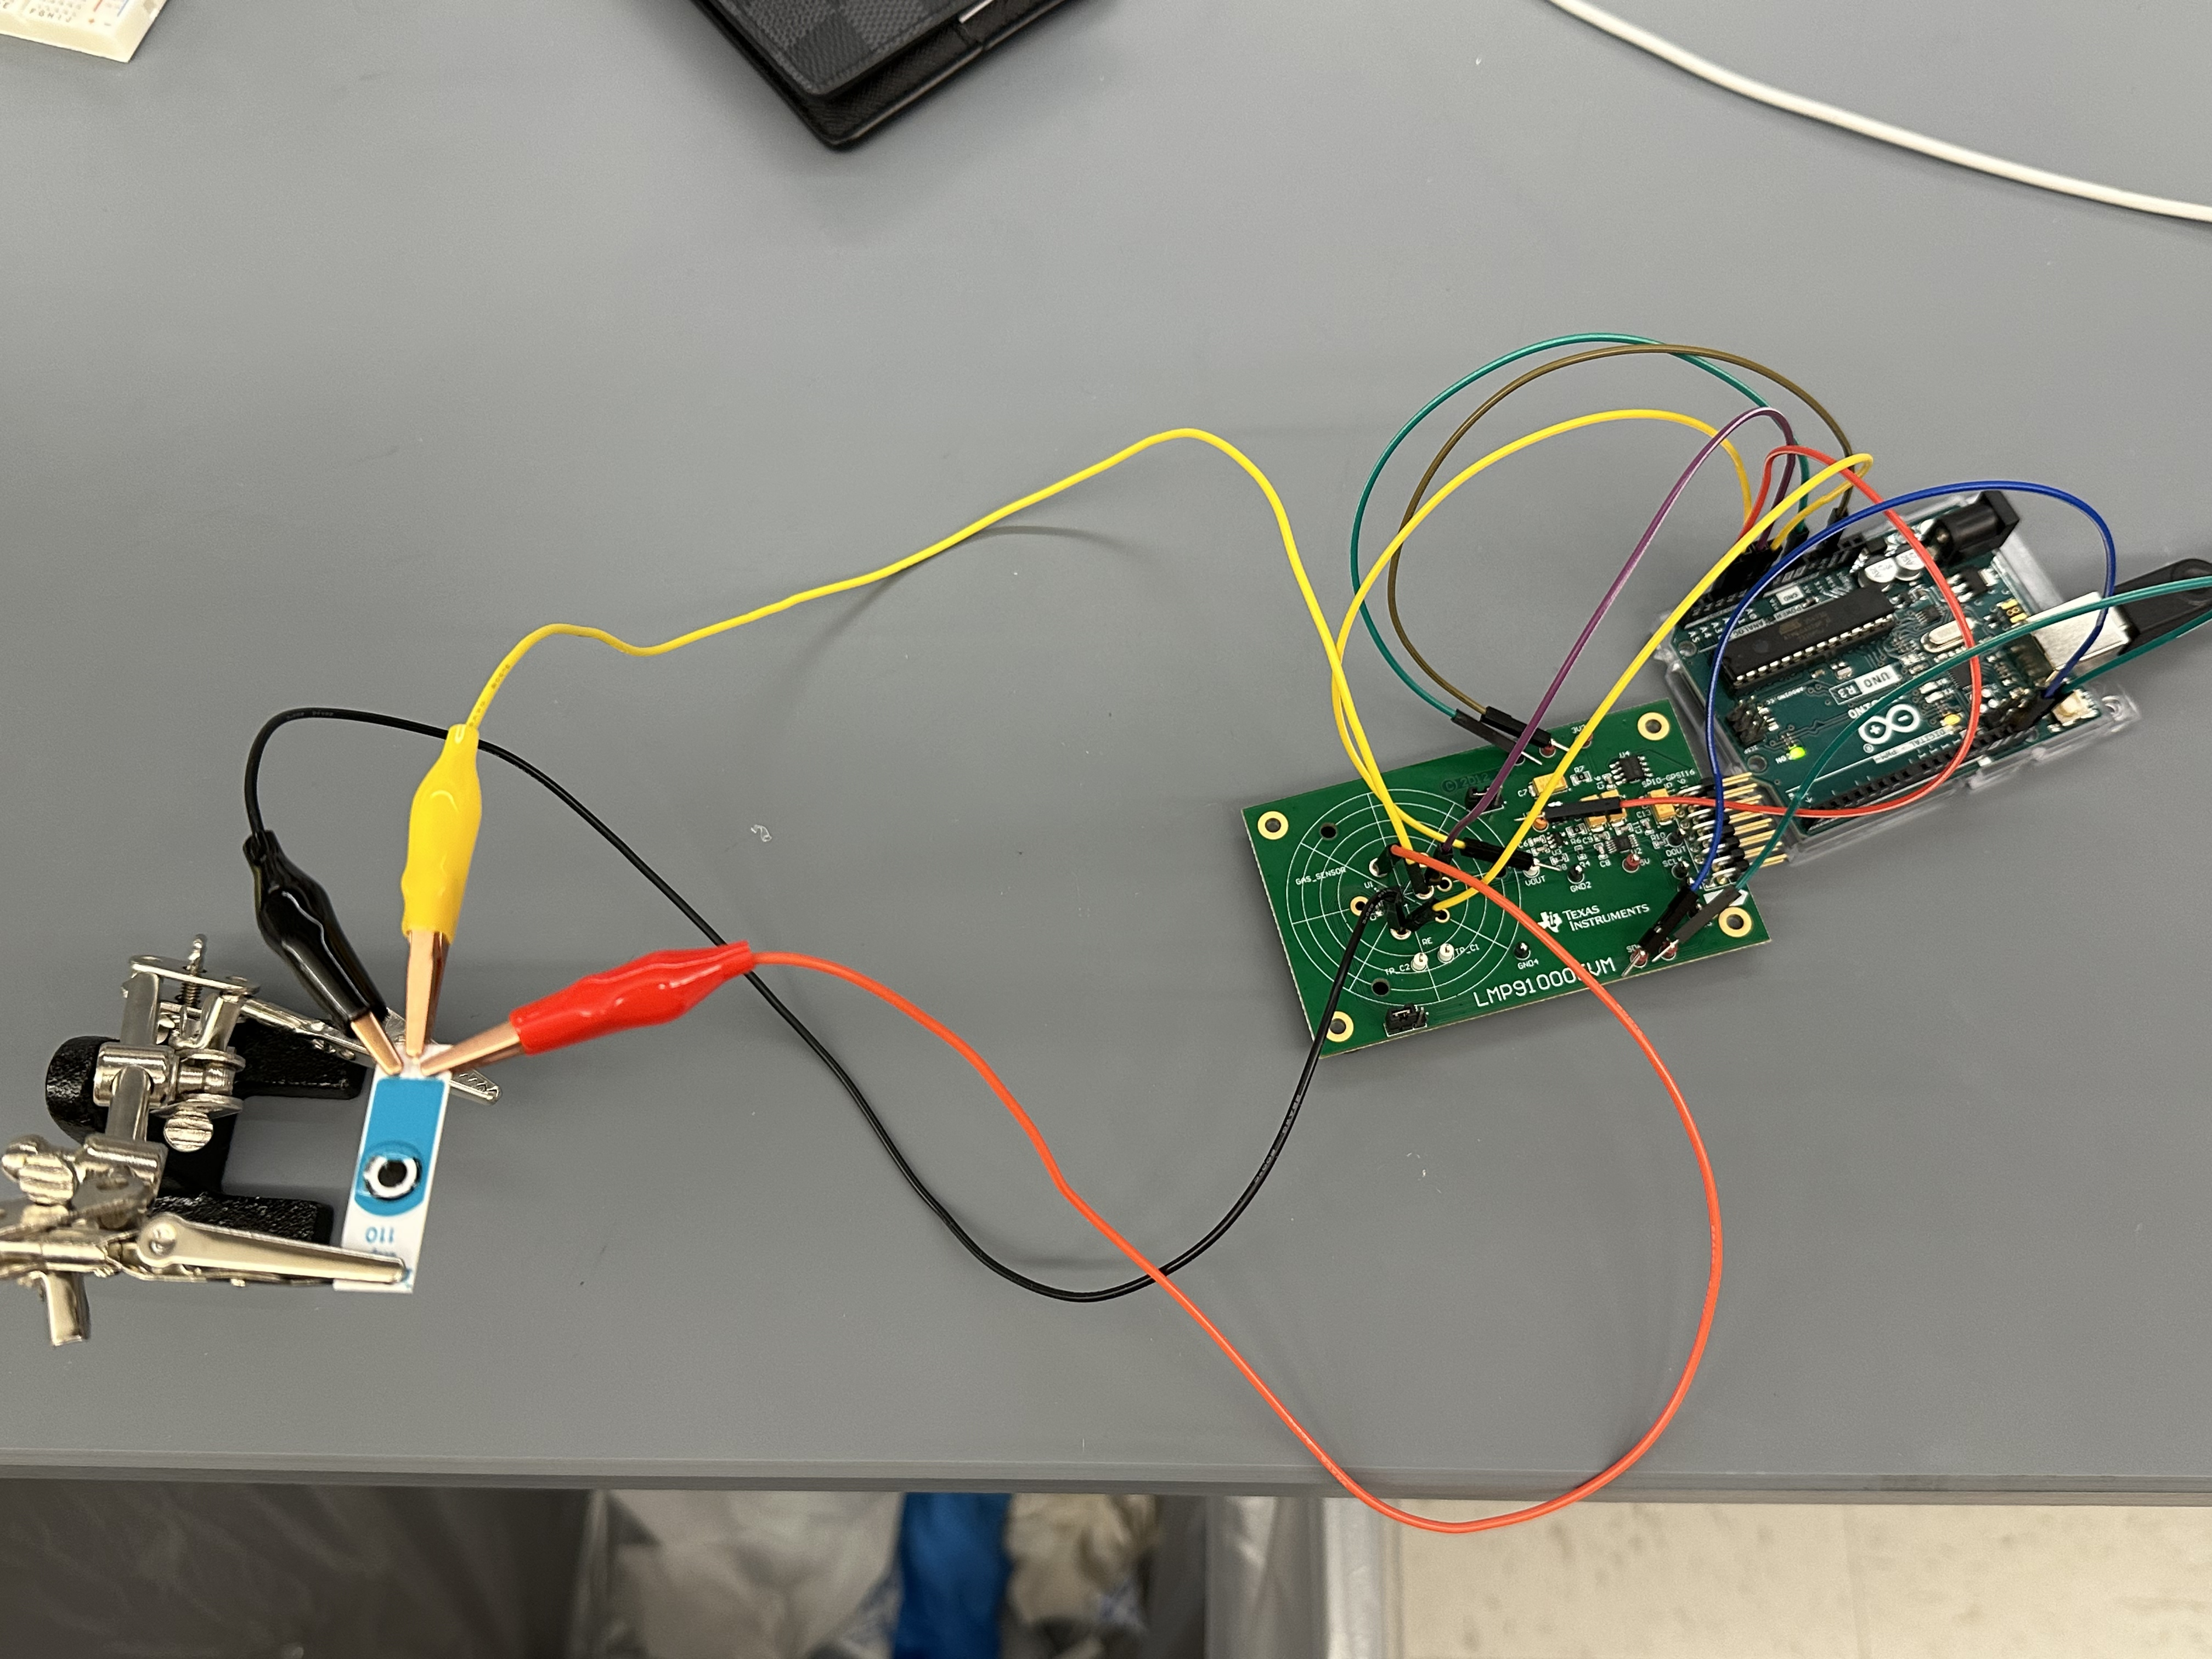
\includegraphics[width=\linewidth]{fig21.jpg}
    \caption{Circuit connection of LMP91000EVM}
    \label{fig21}
\end{figure}

\section{Prototype Arduino sketch}
\label{prototype}

\lstinputlisting{CVtest.ino}

\section{LMP91000EVM benchmark test Arduino sketch}
\label{LMP91000EVM}

\lstinputlisting{LMP91000EVM_CV.ino}


\end{document}